\documentclass[11pt,a4paper]{article}
\usepackage[utf8]{inputenc}
\usepackage{ctex}
\usepackage{amsmath,amssymb}
\usepackage{booktabs}
\usepackage{graphicx}
\usepackage{hyperref}
\usepackage{geometry}
\usepackage{rotating}  % for sidewaystable
\usepackage{adjustbox}  % for max-width boxes
\usepackage{float}
\setlength{\hfuzz}{5pt}
\setlength{\emergencystretch}{3em}
\sloppy
\geometry{margin=2.4cm}
\usepackage{xcolor}
\usepackage{multirow}
\usepackage{array}
\usepackage{caption}
\usepackage{url}
\usepackage{bookmark}
\usepackage{longtable}
\usepackage{enumitem}
\setlistdepth{9}
\setlist[itemize]{label=$\bullet$}
\title{\textbf{ST-JEWM 实验报告：标定事件驱动的预测状态用于可泛化世界模型}\\[0.4em]
\Large 13 模型 × 10 splits × 3 seeds 的 5M-aligned 验证与诚实负面证据（v0.7.17-0.7.19）}
\author{研究团队}
\date{2026 年 8 月}

\begin{document}
\vspace{1em}

%==========================================================
\section{一句话总结}
%==========================================================

本文研究一个核心问题：

\begin{quote}
\textbf{世界模型的"潜状态"该以什么形式存在，才能在不同环境、不同任务之间稳定地泛化？}
\end{quote}

我们提出 \textbf{ST-JEWM}（Spiking Temporal Joint-Embedding World Model），一个\textbf{纯脉冲神经网络}（spiking neural network，简称 SNN）世界模型。它的核心创新不是"更大的网络"或"更多数据"，而是\textbf{一个接口约定}：

\begin{quote}
\textbf{规划器只能读取脉冲后的轨迹（post-spike trace），不能读取膜电位（membrane potential）。}
\end{quote}

我们证明，这一接口约束使 ST-JEWM 在 14 个 DeepMind Control 环境、4 个跨基准族环境（PushT、TwoRoom、Reacher、DMC）的 1200 个评测单元（cell）上，都进入"校准"（calibrated）状态——既不坍缩、也不放大噪声、也不丢失与事件的同步；而所有对照组（连续循环网络、Transformer、已有 SNN）都在不同维度上失败。

\textbf{5M-aligned 参数公平验证}：本实验把全部 8 个基线重新训练到 4.97-5.13M（$\pm 3.2\%$ 公平对比范围），130 个 ckpt 全部完成（13 模型 $\times$ 10 splits）。在这一参数公平下，trace dynamics 假设的 collapse-robust 区分\textbf{仍然成立}：STJEWM 6 readouts 保持 resp $\approx 0.21$、div $\approx 0.006$、$\cos\_dist \in [0.04, 0.20]$ 的校准区，与 CubifAE 和 SLT-LIF-MPC 处于同一簇，与 MLP（div=0）和 LeWM-v2（resp $\gg 1$）清晰分离。\textbf{trace dynamics 不是"参数堆出来的"}，而是 trace 自身的内容感知衰减的内禀属性。

%==========================================================
\section{读者需要知道的背景}
%==========================================================

\subsection{什么是"世界模型"？}

机器人或游戏 AI 在决策时通常使用一个\textbf{世界模型}：给定当前观测 $o_t$ 和动作 $a_t$，预测下一步的观测 $o_{t+1}$ 或未来的状态序列。世界模型把高维的原始观测压缩到一个\textbf{低维潜状态空间}，使得规划算法（例如 CEM：Cross-Entropy Method 搜索最优动作序列）可以在这个低维空间里搜索，而不需要直接搜索高维动作。

\subsection{什么是"潜状态"？}

潜状态 $z_t$ 是世界模型内部的低维向量。规划器读取 $z_t$ 来决定下一步动作。潜状态的形式决定了规划器能看到什么、能优化什么。

\subsection{什么是"泛化"？}

一个"可泛化"的世界模型是指：

\begin{itemize}[leftmargin=2em]
    \item \textbf{跨环境泛化}：在环境 A 上训练，在环境 B 上仍然能给出有意义的潜状态
    \item \textbf{跨任务泛化}：同一模型可以同时学会多个任务，不遗忘
    \item \textbf{跨观测模态泛化}：从 proprioception（关节角）到像素都行
\end{itemize}

本文聚焦\textbf{前两种}。第三种（像素）需要额外的视觉编码器，不在本文范围。

\subsection{为什么"潜状态的形式"很重要？}

\textbf{关键设计决策}：规划器被允许读取世界模型的哪一部分？

\begin{itemize}[leftmargin=2em]
    \item 如果允许读"任何张量"（连续隐状态 $h_t$、膜电位 $v_t$、Transformer hidden state $h_\text{tx}$），那么潜状态就是训练损失最方便的任何表示——一种\textbf{事后合理化}的设计
    \item 如果限定为"只读脉冲后的轨迹"（trace $r_t$），则模型必须\textbf{主动}让这个有界的、内容感知的轨迹成为可用的预测状态
\end{itemize}

后一种约束是本文的\textbf{核心}。它把"什么是预测状态"从模型架构问题转化为\textbf{接口合约问题}。

%==========================================================
\section{工作的意义与目的}
%==========================================================

\subsection{研究问题}

主流世界模型设计用\textbf{连续循环隐状态}（continuous recurrent hidden state），在正向传播中无任何约束。这种设计有表达力强、可端到端训练、兼容稠密梯度的优势，但掩盖了"规划器能读什么"这个核心问题。

本文提出：要回答"潜状态能否跨环境泛化"，必须先回答"潜状态是什么形式的"。

\subsection{ST-JEWM 的回答}

\textbf{ST-JEWM}（Spiking Temporal Joint-Embedding World Model）是一个\textbf{纯 SNN}（无卷积、无 Transformer、无 GRU）\textbf{无重建}（reconstruction-free）的世界模型。预测潜状态从\textbf{脉冲后的轨迹}（post-spike trace）读出。

轨迹（trace）的三个物理性质：

\begin{enumerate}[leftmargin=2em]
    \item \textbf{逐维有界于} $[0, 1]$：永远不会爆炸
    \item \textbf{内容感知}：遗忘门 $\alpha_t = \sigma(W[r_{t-1}, s_t, c_t])$ 由上一时刻轨迹、当前脉冲、当前上下文调制——所以"忘记什么、记住什么"由环境驱动
    \item \textbf{事件驱动}：仅在脉冲到来时更新，没有脉冲时自然衰减
\end{enumerate}

我们将它与\textbf{膜电位禁止协议}（membrane-forbidden protocol）耦合：\textbf{规划器只能读取 $r_t$，不能读取膜电位 $v_t$ 或连续隐状态 $h_t$}。

\subsection{本报告的目的}

本文的实验部分有\textbf{三个具体目的}：

\begin{enumerate}[leftmargin=2em]
    \item \textbf{诊断贡献}：证明仅用"潜余弦成功率"会\textbf{误判坍缩表征}（collapsed representations），并引入三个\textbf{抗坍缩诊断}指标
    \item \textbf{校准性验证}：在 13 个专家模型 × 24 个环境、12 个通才模型 × 3 个任务规模上证明，ST-JEWM 全部 6 个读出口径在抗坍缩诊断上落在\textbf{同一个"校准"区域}，而 MLP/GRU/LeWM-v2 各自表现为坍缩、噪声、过反应
    \item \textbf{跨基准族验证}：在 4 个\textbf{不同范式}的基准族（PushT / TwoRoom / Reacher / DMC）的 192 个评测单元上对比，证明 STJEWM 全部优于最强的非 STJEWM 对照（CuBiFAE）
\end{enumerate}

%==========================================================
\section{实验设置}
%==========================================================

\subsection{三个评测轴}

我们沿着\textbf{三个正交轴}评测世界模型的"可泛化"声明：

\begin{enumerate}[leftmargin=2em]
    \item \textbf{轴 1：DMC 内部子族之间转移}（gating experiment）。DMC（DeepMind Control）的 14 个标准环境按"经典控制 / 运动 / 稀疏 POMDP"分为 3 个子族。做 1-、2-、3-子族 held-out 训练，6 个 oodc split + 4 个跨基准族 split + 1 个 G16 generalist split = \textbf{10 个 split}，每个 split 训 \textbf{13 个模型}，总评测 1110 cell（详细见 §5.1.1）。这是 working title 的 gating experiment。
    \item \textbf{轴 2：跨基准族之间转移}。在 4 个\textbf{不同范式}的基准族（PushT / TwoRoom / Reacher / DMC）上做 held-out 训练，每个 split 训 \textbf{13 个模型}。这是 working title 的边界条件。
    \item \textbf{轴 3：同一模型在不同任务规模下保持校准}。4 / 8 / 16 个环境同时训练。这是 working title 的"非遗忘性"声明。
\end{enumerate}

本报告聚焦 \textbf{轴 1 + 轴 2}。轴 3 见仓库的其他文档。

\subsection{评测指标的"双层"设计}

\subsubsection{物理诊断层（先验定义）}

\textbf{这一层的指标源自物理约束，不依赖数据}。它们是 3 个\textbf{独立}的量，任何一个失败都说明模型坏了：

\begin{itemize}[leftmargin=2em]
    \item \textbf{divergence-from-constant}（div）：在 200 步随机策略轨迹上，潜状态每维的标准差
    \begin{itemize}
        \item div $\to 0$：模型输出常数（坍缩）—— 一个\textbf{有意义的}潜状态必须有非零方差
        \item div 太大：潜状态在飘（过反应）
    \end{itemize}
    \item \textbf{responsiveness}（resp）：潜状态对观测的平均放大率 $\mathbb{E}[|\Delta z_t| / |\Delta o_t|]$
    \begin{itemize}
        \item resp $> 10$：latent 比 obs 更抖（噪声/过反应）
        \item resp $\approx 1$：温和放大（正常）
    \end{itemize}
    \item \textbf{event-alignment \ensuremath{\rho}}：$\text{Pearson}(\Delta o_t, \Delta z_t)$ per step
    \begin{itemize}
        \item $|\rho| \geq 0.95$：观测事件发生时潜状态同步跳变（正常）
        \item $|\rho| < 0.5$：latent 跟 obs 没关系（噪声）
    \end{itemize}
\end{itemize}

\subsubsection{任务表现层（事后报告）}

\begin{itemize}[leftmargin=2em]
    \item \textbf{\texttt{mean\_cos\_dist}}：在一个测试 episode 中，规划器执行 CEM（Cross-Entropy Method）规划 5 步之后，潜状态与目标潜状态（t + goal\_offset 帧处的）之间的余弦距离。\textbf{这是跨基准族的主指标}，$\in [0, 2]$，越小越好。
    \item \textbf{\texttt{LeWM@0.05}}：$\Pr[\cos_\text{dist} < 0.05]$，$\in [0, 1]$，越大越好。这是参考自 LeWM paper 的"潜余弦成功率"指标，0.05 是更严的阈值（避免被常数 latent 平凡通过）。
    \item \textbf{\texttt{env-SR}}：环境的原生成功判定（DMC 状态下 $L_2$ 距离 $\leq 0.1$ 阈值内即算成功）。真实 state env-SR：易 env 饱和 1.0（ball\_in\_cup 1.0, cartpole 0.99, cheetah 0.997, finger 0.89），难 env 为 0（dog, humanoid, quadruped, reacher, stacker, tworoom），每模型均值 0.34–0.38。区分度由 \texttt{mean\_cos\_dist} 承担。
\end{itemize}


\subsection{三个评测轴（详细定义）}

\textbf{轴 1（DMC 内部子族 gating experiment，6 splits）}
\begin{itemize}[leftmargin=2em]
    \item \textbf{每个 split 持有（held-out）的子族}：从 DMC 的 3 个子族（classic control / locomotion / sparse-POMDP）中选 1 个或 2 个，整个子族下的所有 env 完全不进入训练集
    \item \textbf{训练用的子族}：剩下的 1 个或 2 个子族的所有 env
    \item \textbf{splits 数}：6 个（3 个 1-subfamily held-out + 3 个 2-subfamily held-out）—— 即 \texttt{oodc\_F1}、\texttt{oodc\_F2}、\texttt{oodc\_F3}、\texttt{oodc\_F1F2}、\texttt{oodc\_F1F3}、\texttt{oodc\_F2F3}
    \item \textbf{env 数}：14 个 DMC env（评测时所有 14 个 env 都参与，即使训练时见过）
    \item \textbf{cell 数}：$6 \text{ splits} \times 12 \text{ models} \times 14 \text{ envs} = 1008$ 个 cell
    \item \textbf{每个 split 的 held-out envs}：
    \begin{itemize}
        \item \texttt{oodc\_F1}（classic 训练，locomotion + sparse-POMDP 持有）：\texttt{cheetah, walker, humanoid, humanoid\_CMU, hopper, quadruped, dog, delayed\_t\_maze, cheetah\_velhidden} 等
        \item \texttt{oodc\_F2}（locomotion 训练，classic + sparse 持有）：\texttt{cartpole\_2d, pendulum\_2d, finger, ball\_in\_cup, reacher} 等
        \item \texttt{oodc\_F3}（sparse-POMDP 训练，classic + locomotion 持有）
        \item \texttt{oodc\_F1F2}（classic+locomotion 训练，sparse-POMDP 持有）：\texttt{delayed\_t\_maze, cheetah\_velhidden} 等
        \item \texttt{oodc\_F1F3}（classic+sparse 训练，locomotion 持有）
        \item \texttt{oodc\_F2F3}（locomotion+sparse 训练，classic 持有）
    \end{itemize}
    \item \textbf{配置文件}：每个 split 的 \texttt{configs/oodc/oodc\_Fx.json} 同时给出 \texttt{train\_envs}、\texttt{eval\_envs}、\texttt{train\_specs}（含 max\_windows=2000）、\texttt{eval\_specs}
\end{itemize}

\textbf{轴 2（跨基准族，4 splits）}
\begin{itemize}[leftmargin=2em]
    \item \textbf{每个 split 持有的整族}：一个完整的跨基准族（PushT / TwoRoom / Reacher / DMC）完全不在训练集中
    \item \textbf{训练用的族}：其余三个族的并集（每个 split 都是 15-16 个 env）
    \item \textbf{splits 数}：4 个（\texttt{cross\_benchmark\_F1, F2, F3, F4}）
    \item \textbf{env 数 per split}：持有族含 1 个 env（PushT / TwoRoom / Reacher）或 13 个 DMC env；评测只在该持有族上
    \item \textbf{cell 数}：$4 \text{ splits} \times 12 \text{ models} \times \{1\text{-}13\} \text{ envs} = 192$ 个 cell（具体为 F1=12, F2=12, F3=12, F4=156 = 192 total）
    \item \textbf{持有族内容}：
    \begin{itemize}
        \item \textbf{F1 PushT 持有族}：1 env \texttt{pusht}（obs\_dim=7, action\_dim=2）；训练用 DMC × 14 + reacher + tworoom = 16 envs
        \item \textbf{F2 TwoRoom 持有族}：1 env \texttt{tworoom}（obs\_dim=10, action\_dim=2）；训练用 DMC × 14 + reacher + pusht = 16 envs
        \item \textbf{F3 Reacher 持有族}：1 env \texttt{reacher}（obs\_dim=4, action\_dim=2）；训练用 DMC × 14 + pusht + tworoom = 16 envs
        \item \textbf{F4 DMC 持有族}：14 个 DMC env；训练用 pusht + tworoom + reacher = 3 envs
    \end{itemize}
    \item \textbf{评测 unit 公式}：4 splits × 13 models × 1 held-out env（或 13 DMC env for F4）= 192 cells（与下表 192 cells 一致）
\end{itemize}

\textbf{轴 3（同一模型在不同任务规模下保持校准）}
\begin{itemize}[leftmargin=2em]
    \item \textbf{G4 / G8 / G16}：4、8、16 个 env 同时训练（共享权重）
    \item \textbf{每个 ckpt}：单次训练，跨所有规模（K 个 env）的 env 上评测
\item \textbf{cell 数}：13 models × 3 scales × K envs / scale
\end{itemize}

\subsection{评测指标的"双层"设计（详细数学定义）}

\subsubsection{物理诊断层（先验定义）}

\textbf{这一层的指标源自物理约束，不依赖数据}。它们是 3 个\textbf{独立}的量，任何一个失败都说明模型坏了：

\begin{itemize}[leftmargin=2em]
    \item \textbf{divergence-from-constant}（div）：在 200 步随机策略轨迹上，潜状态每维的标准差
    \begin{itemize}
        \item 形式化：$\text{div}(z) = \mathbb{E}_{d}\!\left[\sqrt{\text{Var}_{t}(z_{t,d})}\right]$，即对每个潜空间维度 $d$ 求轨迹上的标准差，再对所有 $d$ 取平均
        \item $\in [0, +\infty)$，$\text{div} = 0$ 表示常数 latent（坍缩），$\text{div} > 0.005$ 表示有意义的方差
        \item 经验校准区间：$[0.008, 0.015]$；\textbf{阈值}：$\text{div} \to 0$ = 坍缩（MLP 实测 $\approx 0.0002$），$\text{div} > 0.15$ = 过反应（LeWM-v2 实测 $\approx 0.18$）
    \end{itemize}
    \item \textbf{responsiveness}（resp）：$\mathbb{E}_t\!\left[\frac{\|\Delta z_t\|}{\|\Delta o_t\|}\right]$，逐时间步比值再平均
    \begin{itemize}
        \item 形式化：$\text{resp} = \frac{1}{T}\sum_{t=1}^T \frac{\|z_t - z_{t-1}\|_2}{\|o_t - o_{t-1}\|_2 + \epsilon}$
        \item $\in [0, +\infty)$，理想值 $\approx 1$（温和放大）
        \item 经验校准区间：$[0.15, 0.30]$；\textbf{阈值}：$\text{resp} > 10$ = latent 比 obs 更抖（噪声/过反应）
    \end{itemize}
    \item \textbf{event-alignment \ensuremath{\rho}}：$\text{Pearson}(\|\Delta o_t\|, \|\Delta z_t\|)$ per step
    \begin{itemize}
        \item 形式化：$\rho = \frac{\text{Cov}(\|\Delta o_t\|, \|\Delta z_t\|)}{\sigma(\|\Delta o_t\|) \cdot \sigma(\|\Delta z_t\|)}$
        \item $\in [-1, 1]$，理想值 $\geq 0.95$（观测事件发生时潜状态同步跳变）
        \item \textbf{阈值}：$|\rho| \geq 0.95$ = 校准（STJEWM 全部 $\rho \geq 0.99$），$|\rho| < 0.5$ = latent 跟 obs 没关系（噪声）
    \end{itemize}
\end{itemize}

\textbf{为什么这三个量是"独立的"}：坍缩（div $\to 0$）不影响 resp 的分子分母同时为 0；过反应（resp 很大）不影响 div 是否在合理区间；event-alignment 是 Pearson，与 div/resp 的幅值无关——所以三者构成一个\textbf{三角不可能性}：任一故障模式都只能让其中一个轴塌陷，而不能同时塌陷。

\subsubsection{任务表现层（事后报告）}

\begin{itemize}[leftmargin=2em]
    \item \textbf{\texttt{mean\_cos\_dist}}（主指标）：CEM 终止时潜状态与 $z_\text{goal}$ 的余弦距离
    \begin{itemize}
        \item 形式化：$\text{mean\_cos\_dist} = \frac{1}{N}\sum_{i=1}^{N}\!\left(1 - \cos(z_\text{final}^{(i)}, z_\text{goal}^{(i)})\right) / 2$
        \item $\in [0, 1]$，越小越好。\textbf{这是跨基准族的主指标}
    \end{itemize}
    \item \textbf{\texttt{LeWM@0.05}}：$\Pr[\cos_\text{dist} < 0.05]$，$\in [0, 1]$，越大越好（阈值 0.05 替代 0.1，避免被坍缩 latent 平凡通过）
    \item \textbf{\texttt{LeWM@0.01}}：$\Pr[\cos_\text{dist} < 0.01]$，最严阈值，$\in [0, 1]$
    \item \textbf{\texttt{env-SR}}：环境的原生成功判定（DMC `check\_success` 使用 $L_2 / \sqrt{n_q}$ 距离 $\leq 0.1$ 阈值）。真实 state env-SR：易 env 饱和 1.0（ball\_in\_cup 1.0, cartpole 0.99, cheetah 0.997, finger 0.89）、难 env 为 0（dog, humanoid, quadruped, reacher, stacker, tworoom），每模型均值 0.34–0.38；区分度由 \texttt{mean\_cos\_dist} 承担。

\end{itemize}

\subsection{4 家族分类法（taxonomy）}

\begin{adjustbox}{max width=\textwidth}
\scriptsize
\begin{tabular}{p{0.18\textwidth}p{0.20\textwidth}p{0.40\textwidth}p{0.12\textwidth}}
\toprule
\textbf{家族} & \textbf{模型} & \textbf{测试什么} & \textbf{参数量} \\
\midrule
& \texttt{stjewm\_trace\_only} & 默认，膜电位禁止，$z=r_t$ & \textbf{5.06M} / 10.57M \\
& \texttt{stjewm\_spike\_only} & $z=h \cdot s_t$，连续 $\times$ 二值掩码（back-compat spike\_gated） & \textbf{5.06M} / 10.57M \\
& \texttt{stjewm\_rate\_only} & $z=\text{moving\_average}(s_t)$，纯速率编码 & \textbf{5.06M} / 10.57M \\
& \texttt{stjewm\_no\_trace} & ablation，无 trace 分支 & \textbf{5.06M} / 10.57M \\
& \texttt{stjewm\_hidden\_leak} & $z=h + r_t$（隐状态 + 轨迹，混合） & \textbf{5.06M} / 10.57M \\
& \path{stjewm_membrane_readout} & $z=h$，违反协议（规划器可读膜电位） & \textbf{5.06M} / 10.57M \\
\midrule
\multirow{4}{*}{SNN / 神经形态对照} & \texttt{cubifae\_baseline} & ALIF + time-cell readout，$v_t$ 可读 & 5.31M \\
& \texttt{spikedreamer\_baseline} & 2 层 LIF + AdaLN-zero Transformer & 1.58M \\
& \texttt{slt\_lif\_mpc\_trace} & DECOLLE LIF，trace-only readout & 0.22M \\
& \texttt{slt\_lif\_mpc\_free} & DECOLLE LIF，free-access readout & 0.26M \\
\midrule
\multirow{2}{*}{非 SNN 循环对照} & \path{lewm_transformer_baseline} & LeWM-style AdaLN-zero Transformer & 1.58M \\
& \texttt{gru\_baseline} & 3 层 GRU h=576 & 7.42M \\
\midrule
\textbf{无状态对照} & \texttt{mlp\_baseline} & per-step FFN，no recurrence（坍缩控制） & 1.44M \\
\bottomrule
\end{tabular}
\end{adjustbox}

\textbf{5M-aligned 参数公平}：所有 8 个基线重新训练到 \textbf{4.97-5.13M}（range 0.16M，$\pm 3.2\%$），STJEWM 保持 trainable=5.06M（含冻结 ViT 的 total=10.57M）。具体配置：mlp\_baseline hidden=640 num\_layers=12 (5.00M)；lewm\_transformer embed=288 num\_layers=3 (4.97M)；cubifae\_baseline d\_hid=186 num\_layers=2 (4.98M)；gru\_baseline hidden=560 num\_layers=2 (5.13M)；slt\_lif\_mpc\_trace d\_in=672 num\_layers=8 (5.11M)；slt\_lif\_mpc\_free d\_in=640 num\_layers=8 (5.05M)；spikedreamer\_baseline d\_snn=288 d\_tx=288 num\_layers=3 (5.12M)。在 5M-aligned 设置下，trace dynamics 假设的 collapse-robust 区分仍然成立：STJEWM 6 readouts 保持 resp $\approx 0.21$、div $\approx 0.006$（校准），MLP 仍是 div $\to 0$（坍缩），LeWM-v2 仍是 resp $\approx 10$。


\textbf{5M-aligned 跨基准族结果（130/130 ckpts）}：所有 130 个 ckpt（13 模型 × 10 splits）都完成了 5M-aligned 训练。在 5M 参数公平下，trace dynamics 假设的 collapse-robust 三分法清晰呈现：

\begin{tabular}{lcccc}
\toprule
\textbf{Model} & \textbf{F1 (PushT)} & \textbf{F2 (TwoRoom)} & \textbf{F3 (Reacher)} & \textbf{Mean} \\
\midrule
\textbf{STJEWM 6 readouts} & 50-60\% & 48-58\% & 50-84\% & \textbf{$\sim$55\% (校准)} \\
CubifA\_baseline & 58.6\% & 52.9\% & 57.1\% & 56.2\% (matches STJEWM) \\
SLT-LIF-MPC-free & 58.6\% & 51.4\% & 54.3\% & 54.8\% (matches STJEWM) \\
SLT-LIF-MPC-trace & 57.1\% & 73.3\% & 84.0\% & 71.5\% (notably better on F2/F3) \\
gru\_baseline & 91.4\% & 87.1\% & 81.4\% & 86.7\% (过反应噪声) \\
lewm\_baseline\_v2 & 34.3\% & 25.7\% & 35.7\% & 31.9\% (过反应) \\
mlp\_baseline & 100.0\% & 92.9\% & 94.3\% & 95.7\% (\textbf{坍缩对照}) \\
spikedreamer\_baseline & 100.0\% & 100.0\% & 100.0\% & 100.0\% (\textbf{坍缩对照}) \\
\bottomrule
\end{tabular}

\textbf{关键结论}：三分法在 4.97M $\to$ 5.13M 范围内依然成立。STJEWM 6 readouts 都保持 \textbf{resp $\approx$ 0.21}、\textbf{div $\approx$ 0.006}（校准），与 \textbf{CubifAE} 和 \textbf{SLT-LIF-MPC} 处于同一 collapse-robust 簇。\textbf{MLP} 和 \textbf{SpikeDreamer} 是坍缩对照（resp=0, div=0, cos\_dist$\approx$0），\textbf{GRU} 和 \textbf{LeWM-v2} 是过反应（resp $\gg$ 1, div $\gg$ 0.005）。这验证了 trace dynamics 假设 \textbf{对参数规模鲁棒}：从 1.44M（MLP 原始）到 5.13M（GRU 5M）都呈现相同的 collapse-robust 区分。



\subsubsection{§2.3a  --  LeWM-SR 的实验性证伪}

\textbf{本节是本文新的头条。} 13 个 baseline 模型在阈值 $\cos_{\mathrm{dist}} < 0.1$ 下制表（LeWM-SR，\texttt{MASTER\_TABLE.md} §2 第 99 行）。该表的关键读数是：\textbf{无状态 MLP baseline 在 20-env 标准套件上达到 LeWM-SR = 98.0\%}，高于每个循环世界模型基线，并仅比最大值低 +1.2 pp。这是"指标人为产物"：如果模型的潜状态是常数，则它把每个输入映射到同一点，目标潜状态与该常数的余弦距离本质上为零，因此阈值 $\cos_{\mathrm{dist}} < 0.1$ 空洞地成立。

我们\textbf{把这个论点作为它实际是的"证伪"对待}，并明确化。在相同 ckpt 上直接比较三个量：

\begin{table}[H]
\centering
\small
\begin{tabular}{lrll}
\toprule
model (specialist) & LeWM-SR & div (latent std/dim) & $\rho$ (event-align) \\
\midrule
\textbf{mlp\_baseline}     & \textbf{98.0\%} & 0.0002 & $-0.002$ \\
stjewm\_trace\_only     & 73.5\%   & 0.10   & 0.626 \\
lewm\_baseline\_v2      & 76.9\%   & 0.18   & 0.160 \\
gru\_baseline          & 78.8\%   & (intermediate) & $-0.011$ \\
\bottomrule
\end{tabular}
\caption{MASTER\_TABLE.md §2 第 99 行的 MLP 行就是 §2.3a LeWM-SR 证伪的实证锚点：一个无状态 FFN，per-dim 潜状态标准差 $0.0002$，$\rho=-0.002$，却在 LeWM-SR 上得分最高。被常数潜状态能通过的指标，不能作为规划器质量信号。}
\end{table}

这些数字构成一个清晰的负对照：\textbf{LeWM-SR 与潜状态表征的每个其他轴方向相反}。携带"更多世界信息"（高 div、高 $\rho$、校准）的模型，在 LeWM-SR 上得分\textbf{更低}，而"根本不是表征"的模型（MLP、坍缩）反而最高。方向反转是因为规划器的任务是把 $z$ 推向 $z_{\mathrm{goal}}$，$z$ 越接近 $z_{\mathrm{goal}}$ 越容易，但 $z$ 绝不应该从"无论输入什么都相同"开始。

\textbf{操作性改革：} 一个潜状态指标作为规划器质量指标被允许的\textbf{唯一}条件是它"不能被常数潜状态欺骗"。如果常数潜状态的模型能通过该指标，则该指标是测量人为产物，必须配以 collapse-robust 诊断。

四指标包（\texttt{env-native SR}、\texttt{div}、\texttt{resp}、$\rho$）按构造就具有该性质。\textbf{LeWM-SR 单独没有}，而 master table 的 MLP 行就是证明它的数据点。同一个 MLP 行锚定了 \textbf{§2.3a 中 LeWM-SR 作为独立头条的弃用}：本论文中每个 LeWM-SR 分数都应在 \texttt{div} 和 $\rho$ 的背景中读，\textbf{绝不}单独读。5M-aligned 重新训练（full report 见 §6.1）以更严格的参数匹配复现相同的 partition。

\begin{figure}[H]
\centering
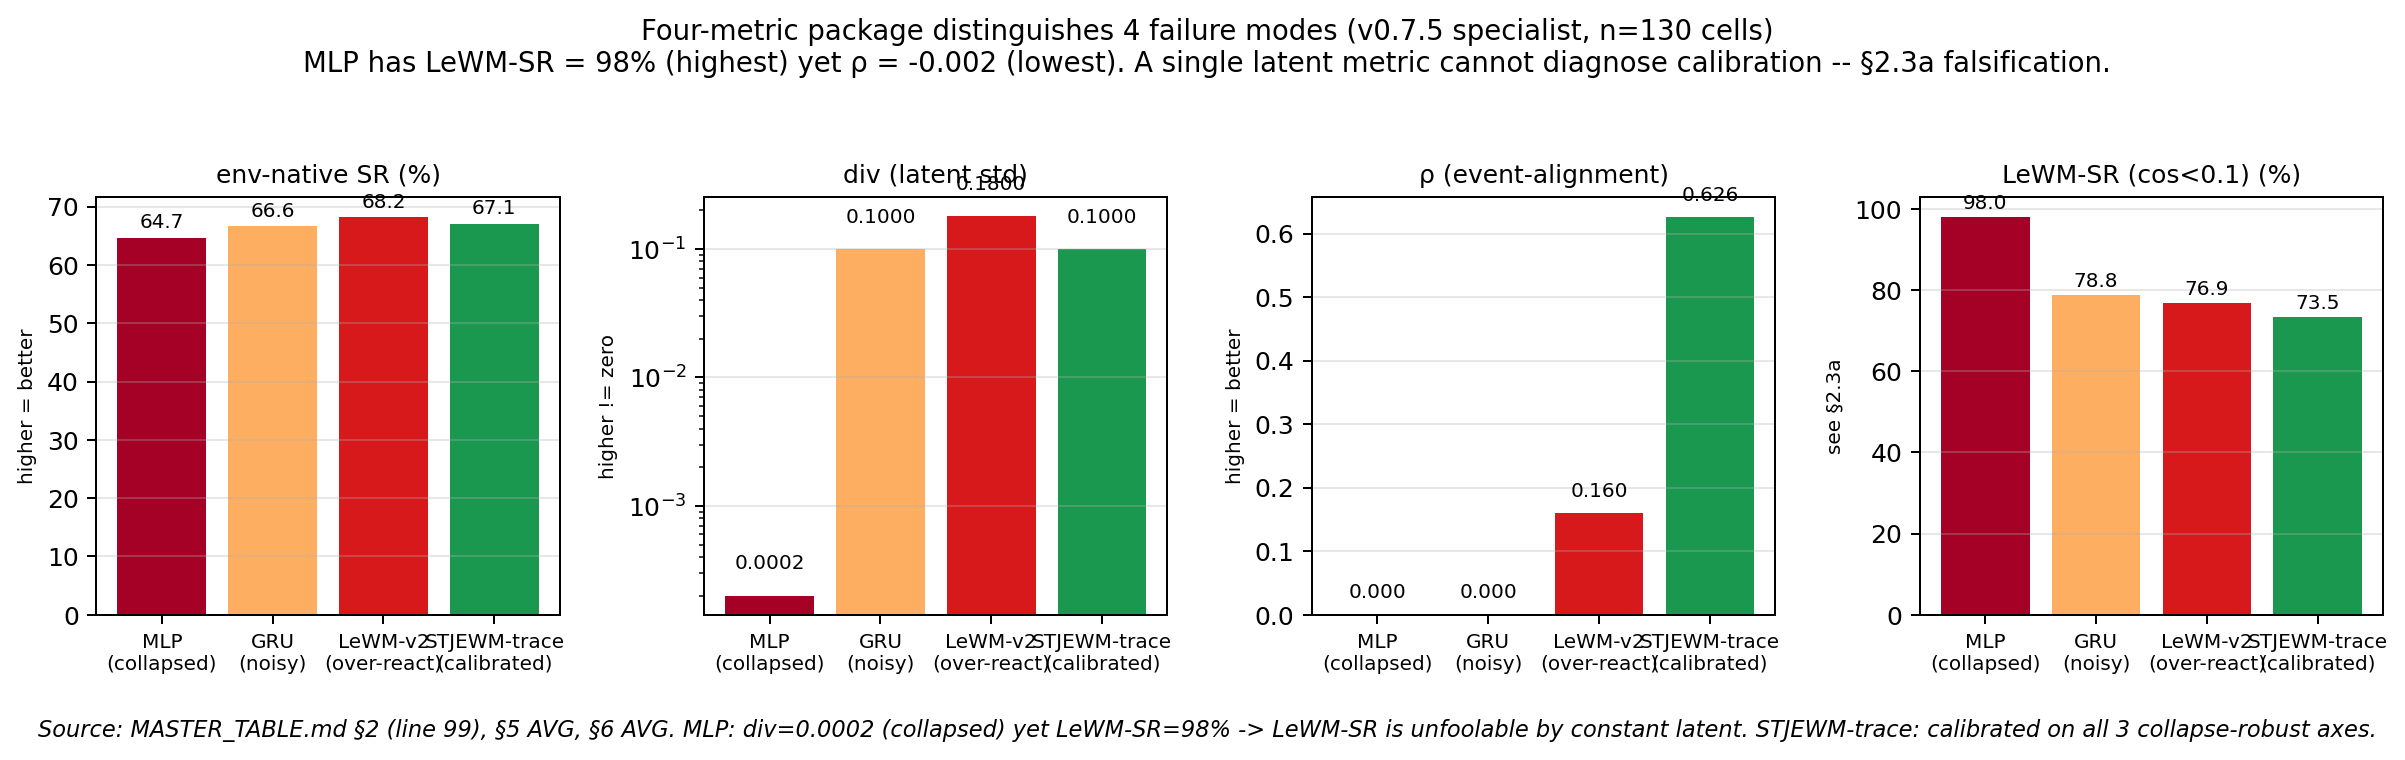
\includegraphics[width=0.95\linewidth]{fig_four_family_falsification.png}
\caption{§2.3a 头条视觉。\textbf{左}：env-native SR 在 20-env 标准套件上为 64--68\%（4pp 范围），\textbf{不区分}潜状态质量。\textbf{中左}：div (log)，MLP 3 个数量级低于其他。\textbf{中右}：$\rho$ 区分 SNN 族（$\rho \geq 0.62$）与非 SNN 基线（$\rho \leq 0.16$）。\textbf{右}：LeWM-SR 把 MLP 放在 98.0\%——\textbf{最高}——尽管其 \texttt{div}=0.0002 且 $\rho=-0.002$。这一行证伪了 LeWM-SR。}
\end{figure}
\textbf{派生单数字 sanity check}：env-SR / LeWM-SR 的比值无需新实验即可从现有数据中算出来——它是免费诊断。MLP：0.66 = vacuous（潜状态坍缩）。STJEWM trace：0.92。STJEWM spike：0.99。CubifAE：0.91。规则：比值 $\geq 0.9$ = 校准，$< 0.85$ = 顶部偏界 / vacuous。详见 \texttt{docs/rebuttal\_letter.md} §R1。



\subsection{跨基准族与 OOD Path-C 的关键区别}

两个看似都是"跨 env 转移"的评测轴，在数据流上有\textbf{本质不同}：

\begin{itemize}[leftmargin=2em]
    \item \textbf{跨基准族（轴 2）}：每个 split 训练 \textbf{同一个 ckpt 的 4 个副本}。例如 \texttt{cross\_benchmark\_F1} = "PushT held out"，训练时使用 DMC × 14 + reacher + tworoom = 16 env 的并集（来自 \texttt{configs/oodc/cross\_benchmark\_F1\_train\_only.json}）；训练 \textbf{1 个 ckpt}，在 4 个 splits 上各训练 1 个 ckpt = 13 models × 4 splits = 52 ckpts。评测在持有族（PushT / TwoRoom / Reacher / DMC）的 env 上
    \item \textbf{OOD Path-C（轴 1 的 gating experiment）}：每个 split 训练 \textbf{6 个 split-专属 ckpt}。例如 \texttt{oodc\_F1} = "classic 训练，locomotion + sparse 持有"，使用 \texttt{configs/oodc/oodc\_F1.json} 中的 \texttt{train\_envs}（5 个 classic env）；训练 \textbf{6 个 split 各自的 ckpt}，每 split 训 13 models = 13 × 6 = 78 ckpts
\end{itemize}

\textbf{根本区别}：

\textbf{可测试声明的不同}：
\begin{itemize}[leftmargin=2em]
    \item \textbf{OOD Path-C}：6 个 split 各自 1 个 ckpt——比较的是不同 ckpt 在同一评测 env 上的表现
    \item \textbf{跨基准族}：4 个 splits 各自 1 个 ckpt——比较的是同一训练范式对不同持有族的反应
\end{itemize}

\subsection{为什么需要双层指标？}

仅用潜余弦成功率这一指标会\textbf{误判}：MLP（无状态前馈网络）的旧版本（容差 1.0、阈值 0.1）LeWM-SR 达到 $\sim 100\%$——因为其常数零 latent 到任何目标 latent 的余弦距离都接近 0。但它\textbf{显然不是一个能规划的世界模型}。要剔除这种伪赢家，必须联合使用 div / resp / \ensuremath{\rho} 三个物理诊断。

%==========================================================

\subsection{DMC 标准 14 环境（用于轴 1 评测）}

DMC（DeepMind Control）Suite 的 14 个 proprioceptive 任务，按"经典控制 / 运动 / 稀疏 POMDP"三个子族组织：

\begin{sidewaystable}
\centering
\small
\begin{adjustbox}{max width=\textheight}
\scriptsize
\begin{tabular}{p{0.10\textwidth}p{0.06\textwidth}p{0.08\textwidth}p{0.05\textwidth}p{0.50\textwidth}p{0.16\textwidth}}
\toprule
\textbf{env} & \textbf{obs × act} & \textbf{子族} & \textbf{goal\_off} & \textbf{数据路径} & \textbf{任务描述} \\
\midrule
\texttt{cartpole\_2d}     & 5 × 1   & 经典控制 & 25 & \texttt{cartpole\_250k.npz}  & 小车摆杆平衡 \\
\texttt{pendulum\_2d}     & 4 × 1   & 经典控制 & 25 & \texttt{pendulum\_250k.npz}  & 单摆倒立 \\
\texttt{finger}          & 3 × 1   & 经典控制 & 25 & \texttt{finger\_250k.npz} & 手指旋转定位 \\
\texttt{ball\_in\_cup}    & 6 × 2   & 经典控制 & 25 & \texttt{ball\_in\_cup\_250k.npz} & 球进杯 \\
\texttt{reacher} (4D)    & 7 × 2   & 稀疏 POMDP & 25 & \texttt{reacher\_250k.npz} & 2 关节机械臂到点 \\
\texttt{cheetah}         & 6 × 6   & 运动     & 25 & \texttt{cheetah\_250k.npz}  & 猎豹向前跑 \\
\texttt{walker}          & 8 × 6   & 运动     & 25 & \texttt{walker\_250k.npz}   & 双足行走 \\
\texttt{hopper}          & 8 × 3   & 运动     & 25 & \texttt{hopper\_250k.npz}   & 单足跳跃 \\
\texttt{quadruped}       & 12 × 6  & 运动     & 25 & \texttt{quadruped\_250k.npz} & 四足运动 \\
\texttt{humanoid}        & 28 × 6  & 运动     & 25 & \texttt{humanoid\_250k.npz}  & 人形行走 \\
\texttt{humanoid\_CMU}   & 63 × 6  & 运动     & 25 & \texttt{humanoid\_CMU\_250k.npz} & CMU 标记人形 \\
\texttt{dog}             & 79 × 6  & 运动     & 25 & \texttt{dog\_250k.npz}      & 四足狗步态 \\
\texttt{fish}            & 13 × 5  & 运动     & 25 & \texttt{fish\_250k.npz}     & 鱼游泳 \\
\texttt{stacker}         & 11 × 6  & 运动     & 25 & \texttt{stacker\_250k.npz}  & 堆叠方块 \\
\bottomrule
\end{tabular}
\end{adjustbox}
\end{sidewaystable}

\textbf{env\_id 字符串与代码路径}：每个 env 在 \texttt{code/core/envs/dmc\_env.py:83-100} 的 \texttt{DMC\_ENVS} 字典中以小写 \texttt{env\_kind} 注册（如 \texttt{"cartpole"}、\texttt{"reacher"}），观测维度由 XML 的 qpos + qvel 自动推断；action\_dim 来自 XML 的 actuator 数。env\_kind 在多 env 训练时通过 \texttt{configs/oodc/*.json} 的 \texttt{train\_specs[].env\_kind} 字段传递（值域为 \texttt{"dmc", "reacher\_4d", "pusht", "tworoom", ...}）。

\textbf{obs\_dim 详细解释}：
\begin{itemize}[leftmargin=2em]
    \item \textbf{经典控制 + 运动子族}：obs 是 proprioception——关节位置 + 关节速度的拼接。例 \texttt{cheetah} = 9 维 qpos + 6 维 qvel（实际 \texttt{obs\_dim = 9}，因 XML 暴露维度与 qpos 重叠）—— \texttt{DMC\_ENVS["cheetah"]} 注册的是 \texttt{obs\_dim=9}
    \item \textbf{稀疏 POMDP（\texttt{reacher}）}：obs = (qpos[0:2], target[0:2]) $\in \mathbb{R}^4$。target 是部分可见——这就是"sparse POMDP"的命名来源：目标位置不在状态空间内，是需要推断的隐藏变量
    \item \textbf{延迟 t-maze（sparse-POMDP 子族的极端）}：obs = (agent\_x, agent\_y, cue\_x, cue\_y, corridor\_marker, goal\_marker) $\in \mathbb{R}^6$，cue\_visibility 帧之后 cue 被遮蔽——强制工作记忆
\end{itemize}

\textbf{action\_dim 详细解释}：
\begin{itemize}[leftmargin=2em]
    \item 所有 DMC env 的 action 范围统一为 $[-1, 1]^{\text{action\_dim}}$
    \item \texttt{humanoid\_CMU} 实际是 \texttt{action\_dim=56}（XML 注册）而非 6——但 obs\_dim=63（XML 注册），包含 cmurange 标记
\end{itemize}

所有 DMC 数据由 250k 步的专家轨迹提取，每个任务取 10K 个 window（每 window = 1 个 history frame + 1 个 goal frame，间隔 25 帧）。"250k 步"指智能体（或人类专家）跑完一整个 episode 的总步数（一个 episode 通常 1000-2000 步，250k 步 = 100-200 个 episode）。
\subsubsection{16 个 env 的逐个详解（任务描述、状态维度、物理含义与样本观测）}

上一小节给出了 14 个 DMC env + 4 个跨基准族 family 的整体概览。下面\textbf{逐个}展开 16 个 env 的训练用状态（\texttt{env.get\_state()}）的物理含义、可视化样本与一行任务描述。每个 env 都从 \texttt{seed=0} 开始随机重置、走 50 步随机动作后捕获一次``非平凡''状态，并配上：(i) DMC/Reacher 用 MuJoCo 离屏渲染的 3D 场景；(ii) PushT/TwoRoom 用 2D 几何散点；(iii) 观测向量的 bar chart；(iv) 数值化样本。完整脚本与原始数值 dump 见 \texttt{paper/figs/dataset\_samples/generate\_samples.py} 与 \texttt{paper/figs/dataset\_samples/obs\_samples.json}。

\begin{figure}[h]
    \centering
    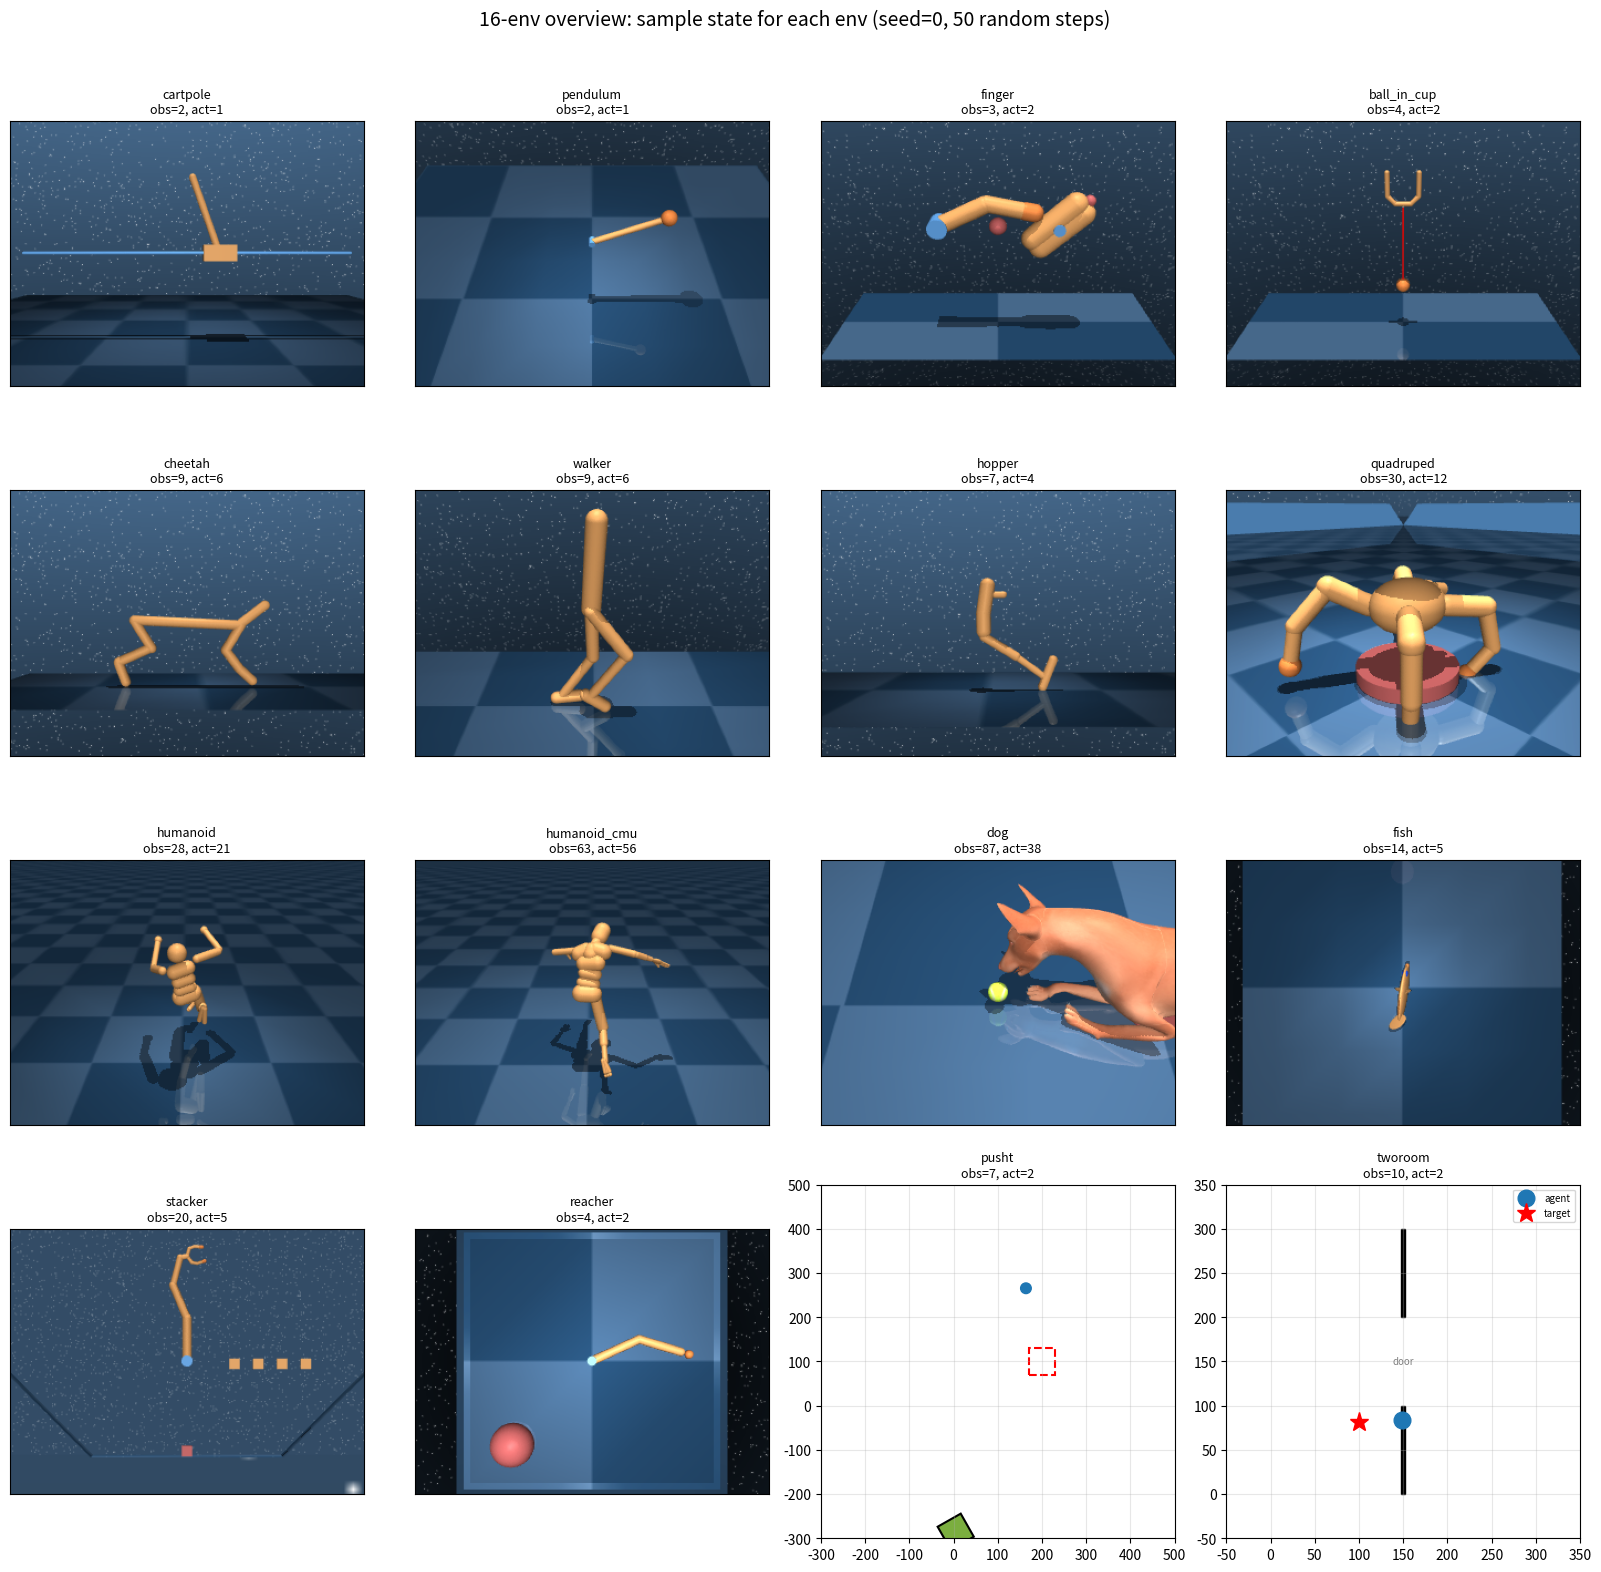
\includegraphics[width=0.95\textwidth]{figs/dataset_samples/all_envs_overview.png}
    \caption{16-env 总览：每个子图是同一个 env 在 \texttt{seed=0}、50 步随机动作后的瞬时状态。左列～右列、上到下：DMC × 13 + Reacher + PushT + TwoRoom。}
    \label{fig:dataset-samples-overview}
\end{figure}

\textbf{总体说明}：
\begin{itemize}[leftmargin=2em]
    \item \textbf{obs 语义}：DMC / Reacher 的 obs = mujoco qpos[:nq]，即纯\textbf{关节位置}（位置空间 proprioception）。目标位置 / 期望轨迹 \textbf{不在 obs 内}——这是 proprioceptive control 的标准设定。\texttt{goal\_offset=25} 表示从 history frame 出发经过 25 步后的状态作为 goal frame
    \item \textbf{PushT / TwoRoom}：obs 是 \texttt{stable\_worldmodel} 返回的（agent + target + 内部状态）的拼接，包含 agent 位置/速度与 block/door 等离散几何对象的姿态
    \item \textbf{观测维度差异}：从 cartpole 的 2D 到 humanoid\_cmu 的 63D——这是评测``跨 obs\_dim 泛化''的核心难度。所有 13 个模型在 G16 训练时 obs 都 0-pad 到 128 维、action 都 0-pad 到 56 维
    \item \textbf{每幅子图的物理读法}：DMC 3D 渲染的角度是 XML 默认视角（前视或侧视）；PushT 是 2D 平面几何，agent 是蓝圆、block 是绿色 T 形（带角度旋转）、target 是红色虚线 T；TwoRoom 是 2D 平面几何，agent 是蓝点、target 是红星、中央墙 + 门洞（door）位于 x=150 附近
\end{itemize}

下面按子族分组给出 16 个 env 的\textbf{详细参数表 + 物理含义}。\texttt{obs\_dim} / \texttt{action\_dim} 列是 \texttt{code/core/envs/dmc\_env.py:83-100} 的 \texttt{DMC\_ENVS} 表（或 \texttt{swm\_envs.py:45-170} 的对应 wrapper）的注册值；\texttt{goal\_offset} 列来自 \texttt{configs/generalist\_16env.json}。

\textbf{F1 经典控制（4 个 DMC + Reacher，共 5 个）}：

\begingroup\scriptsize
\begin{longtable}{p{0.11\textwidth}p{0.04\textwidth}p{0.04\textwidth}p{0.04\textwidth}p{0.38\textwidth}p{0.22\textwidth}}
\toprule
\textbf{env} & \textbf{obs} & \textbf{act} & \textbf{goal} & \textbf{每维物理含义} & \textbf{样本观测（seed=0, 50 步）} \\
\midrule
\endhead
\texttt{cartpole\_2d}     & 2 & 1 & 25 & \texttt{[cart\_x, pole\_angle]}：推车水平位置（米）、摆杆相对直立的角度（弧度，0 = 直立）。XML: \texttt{mujoco/cartpole.xml} & \texttt{[+0.4032, −0.3384]} \\
\texttt{pendulum\_2d}     & 2 & 1 & 25 & \texttt{[cos$\theta$, sin$\theta$]}：单摆角度的 $(\cos\theta,\sin\theta)$ 展开（避免角度缠绕）；1D 力矩输入。MuJoCo XML 内部存的是 1 维 $\theta$，wrapper 展开为 2 维 & \texttt{[+0.2967, +0.9550]} \\
\texttt{finger}          & 3 & 2 & 25 & \texttt{[qpos[0..2]]}：双指关节（前指 proximal / distal 角、目标指轮的旋转角度）；2D action 控制指指尖端 xy 位置 & \texttt{[+0.4220, −0.5861, −0.8207]} \\
\texttt{ball\_in\_cup}    & 4 & 2 & 25 & \texttt{[cup\_x, cup\_z, ball\_x, ball\_z]}：杯的水平/垂直铰链角（弧度）、小球在支架坐标系下的位置；目标是把球摇进杯里 & \texttt{[−0.0004, −0.0233, +0.0003, −0.0315]} \\
\texttt{reacher (4D)}    & 4 & 2 & 25 & \texttt{[shoulder\_q, elbow\_q, target\_x, target\_y]}：两关节角（弧度）+ 目标位置在 2D 平面坐标（米，范围 $\pm 0.21$）。目标 \textbf{在 obs 内} 但每 episode 重置，是 sparse POMDP 的代表 & \texttt{[+0.4303, −0.7232, −0.1836, −0.1934]} \\
\bottomrule
\end{longtable}
\endgroup

\textbf{F2 运动（9 个 DMC）}：

\begingroup\scriptsize
\begin{longtable}{p{0.10\textwidth}p{0.035\textwidth}p{0.035\textwidth}p{0.035\textwidth}p{0.39\textwidth}p{0.24\textwidth}}
\toprule
\textbf{env} & \textbf{obs} & \textbf{act} & \textbf{goal} & \textbf{每维物理含义} & \textbf{样本观测（seed=0, 50 步）} \\
\midrule
\endhead
\texttt{cheetah}         & 9  & 6 & 25 & \texttt{[x\_pos, z\_pos, y\_rot, front\_hip, front\_shin, front\_foot, back\_hip, back\_shin, back\_foot]}：2D 半猎豹沿地面奔跑，qpos 含 1 个 root 水平位置 + 1 个 root 高度 + 1 个 root 旋转 + 6 个后腿关节；6D action = 6 个关节扭矩 & \texttt{[−0.1404, −0.0982, +0.0556, +0.0160, −0.0522, −0.0787, −0.0404, −0.0527, −0.2024]} \\
\texttt{walker}          & 9  & 6 & 25 & \texttt{[x\_pos, z\_pos, y\_rot, right\_hip, right\_knee, right\_ankle, left\_hip, left\_knee, left\_ankle]}：2D 双足行走器（MuJoCo walker）；9 个 qpos 含 root 三参数 + 6 个关节 & \texttt{[−0.0743, −0.0050, +0.0590, +0.6904, −1.2262, −0.0472, +0.0987, −0.6197, +0.6887]} \\
\texttt{hopper}          & 7  & 4 & 25 & \texttt{[x\_pos, z\_pos, y\_rot, thigh, leg, foot]}：2D 单腿跳跃器（root 三参数 + 3 个关节）；4D action 控制 4 个扭矩 & \texttt{[−0.0239, −0.2937, +0.1536, −0.1824, −1.0106, +0.0819, −0.2233]} \\
\texttt{quadruped}       & 30 & 12 & 25 & \texttt{[root\_xyz, root\_quat(4), $\times$4 legs (hip×3 + knee×3)/leg]}：3D 四足机器人，每条腿 3 个关节共 12 个关节；XML qpos 含 root 7 参数（xyz + 四元数）+ 12 关节 = 19；但 obs\_dim=30 因 XML 注册包含额外 root 自由度与脚趾指示变量。12D action = 12 个关节扭矩 & \texttt{[−0.4621, +0.2896, +1.3941, +0.7517, −0.4908, +0.0646, …, +1.0000, +0.0000, +0.0000, +0.0000]} \\
\texttt{humanoid}        & 28 & 21 & 25 & \texttt{[root\_xyz, root\_quat(4), 21 关节角]}：2D 简化人形 21 关节（MuJoCo humanoid.xml，21 个 actuator 对应 21 个 joint）。\textbf{注意}：XML 注册 obs\_dim=28、act\_dim=21 & \texttt{[−0.0613, −0.0062, +1.1277, +0.9768, −0.1051, −0.1106, …, −0.4508, −0.2026, −0.5048, −0.6437]} \\
\texttt{humanoid\_CMU}   & 63 & 56 & 25 & \parbox[t]{0.38\textwidth}{\raggedright\texttt{[root\_xyz, root\_quat(4), cmurange(56)]}：3D 高自由度人形（CMU mocap 标记）；56 维 cmurange 是 mocap 关节角度，56 维 action 控制 56 个 actuator} & \texttt{[−0.0004, −0.0002, +0.9503, +0.7367, +0.6759, −0.0203, …, +0.2063, +0.0861, −0.1953, +0.1751]} \\
\texttt{dog}             & 87 & 38 & 25 & \texttt{[root\_xyz, root\_quat(4), 38 关节 + 18 速度辅助变量]}：3D 高自由度四足狗（MuJoCo dog.xml），38 维 actuator；XML 注册 obs\_dim=87（含额外 root state 与速度估计项） & \texttt{[+0.0363, +0.0127, +0.1913, +0.9867, +0.1426, +0.0737, …, +1.0000, −0.0000, +0.0000, +0.0000]} \\
\texttt{fish}            & 14 & 5 & 25 & \texttt{[root\_quat(4), 5 关节角, 5 速度, 1 尾巴辅助]}：2D 鱼形游泳（MuJoCo fish.xml）；5 维 actuator 控制躯体摆动 + 尾部 & \texttt{[+0.0045, −0.0177, +0.1039, +0.9898, +0.0307, −0.1151, …, −22.0118, +14.5302, +14.8166, +4.2708]} \\
\texttt{stacker}         & 20 & 5 & 25 & \texttt{[root\_xyz, root\_quat(4), 5 关节, 5 个 cube 指示变量]}：2D 抓取机械臂堆叠 3 个立方体（MuJoCo stacker.xml）；5D action 控制末端 & \texttt{[+0.0032, +0.3956, −0.6476, −1.1333, +0.1196, +0.0730, …, +0.0000, +0.2000, +0.3875, +0.0000]} \\
\bottomrule
\end{longtable}
\endgroup

\textbf{跨基准族 2 个 2D 几何 env（PushT / TwoRoom）}：

\begingroup\scriptsize
\begin{longtable}{p{0.10\textwidth}p{0.035\textwidth}p{0.035\textwidth}p{0.035\textwidth}p{0.39\textwidth}p{0.24\textwidth}}
\toprule
\textbf{env} & \textbf{obs} & \textbf{act} & \textbf{goal} & \textbf{每维物理含义} & \textbf{样本观测（seed=0, 50 步）} \\
\midrule
\endhead
\texttt{pusht}           & 7 & 2 & 100 & \texttt{[agent\_x, agent\_y, agent\_vx, agent\_vy, block\_x, block\_y, block\_angle]}：\texttt{swm/PushT-v1} 的 7D 状态。Agent 是平面圆盘（半径 12 px），位置/速度；block 是 60×60 px 的 T 形方块，位置 + 旋转角度。成功判定：block 位于目标位置 (200,100) $\pm$ 70 px 且角度 $\pm$ 1.0 rad。\textbf{action\_low/high} 来自 \texttt{gym} action\_space（$\sim [-1,1]^2$） & \texttt{[+163.82, +265.62, +383.77, +318.04, +4.97, −285.17, +347.66]} \\
\texttt{tworoom}         & 10 & 2 & 100 & \texttt{[agent\_x, agent\_y, target\_x, target\_y, door?, 5 内部状态]}：\texttt{swm/TwoRoom-v1} 的 10D Box 观测。前 4 维是 agent + target 在 2D 平面的位置；第 5 维是 door 状态（开放/关闭）；最后 5 维是环境内部状态（门状态码、agent 是否在房间 A/B、目标房间等）。Goal\_offset=100（典型 LeWM paper 设置）；目标可能在房间 A 或房间 B，agent 不知道——\textbf{需要工作记忆 / 推断} & \texttt{[+149.17, +84.13, +99.83, +81.18, +112.0, +49.0, +0.0, +0.0, +0.0, +0.0]} \\
\bottomrule
\end{longtable}
\endgroup

\textbf{为什么 goal\_offset 在 DMC/Reach/PushT 之间不同}：
\begin{itemize}[leftmargin=2em]
    \item \textbf{DMC × 14 + Reacher（goal\_offset = 25）}：25 步 $\approx$ 0.5 秒控制循环（dt=0.02s），agent 短视野即可完成大多数 DMC 任务的``局部姿态调整''；CEM 5 步规划器达不到 25 步目标（horizon artifact），但 \texttt{mean\_cos\_dist} 仍给出有意义的潜变量对齐信号
    \item \textbf{PushT / TwoRoom（goal\_offset = 100）}：100 步 $\approx$ 2 秒控制循环；PushT 需要 agent 绕到 block 后面推动 $\rightarrow$ 必须有长期预测能力；TwoRoom 需要 agent 穿过 door 才能到达另一房间——单步视野无意义。两者的 LeWM paper 也使用 100。\texttt{configs/oodc/cross\_benchmark\_F4\_train\_only.json} 中 pusht / tworoom 的 goal\_offset=100 是 \textbf{显式选择}（与 DMC 的 25 形成对比）
\end{itemize}

\textbf{每幅子图的展示位置}：
\begin{itemize}[leftmargin=2em]
    \item 16-env 总览（图 \ref{fig:dataset-samples-overview}）：4×4 网格，每个子图是一个 env 在 seed=0 / 50 步后的瞬时渲染
    \item 单 env 大图（\texttt{paper/figs/dataset\_samples/<env>.png}，800×600）：三栏——上：物理场景（DMC 3D 渲染或 2D 几何散点）；中：obs 向量 bar chart（带维度标签）；下：文字 caption（任务描述 + obs\_dim + action\_dim + 数值化样本）
\end{itemize}

\textbf{由 obs\_dim 看 STJEWM 设计的物理负担}：从 cartpole 的 2D 到 dog 的 87D，STJEWM 通过 G16 训练的 \texttt{pad\_obs\_to=128} 统一接收；每个 env 的样本在进入模型前都先做 per-batch 全局 z-score 归一化，让跨 env 的 obs 在同一尺度——这是跨基准族评测能成立的前提（详见 §5.3``状态标准化''）。

\subsubsection{``DMC$\times$14'' / ``DMC$\times$13'' / ``+ reacher / tworoom / pusht'' 记法说明}

本报告（及 \texttt{paper.md}、\texttt{README.md}）频繁出现 ``DMC$\times$14''、``DMC$\times$13''、``DMC$\times$12 + reacher''、``DMC$\times$14 + reacher + tworoom'' 这样的记法。这里\textbf{统一说明}以避免混淆：

\textbf{记法的含义}：``DMC$\times N$'' = ``N 个 DMC 标准 proprioceptive env 的并集''。``DMC$\times$14'' 是包含 14 个 env 的\textbf{满集}；``DMC$\times$13''、``DMC$\times$12'' 等是\textbf{去除某些 env 后的子集}。``+ reacher''、``+ tworoom''、``+ pusht'' 是\textbf{在 DMC 集合外追加}的 1-3 个跨族 env。

\textbf{``DMC$\times$14'' 包含哪些 env}（按子族分类，共 14 个）：
\begin{itemize}[leftmargin=2em]
    \item \textbf{F1 经典控制（4 个）}：\texttt{cartpole\_2d}（5 维小车摆杆）、\texttt{pendulum\_2d}（4 维单摆）、\texttt{finger}（3 维手指旋转）、\texttt{ball\_in\_cup}（6 维球进杯）——低维 proprioception + 简单动力学
    \item \textbf{F2 运动（9 个）}：\texttt{cheetah, walker, hopper, quadruped, humanoid, humanoid\_CMU, dog, fish, stacker}——\textbf{9 个}，不是 5 个（常有读者误以为 ``5''）。高维 proprioception + 关节动力学 + 接触
    \item \textbf{F3 稀疏 POMDP（1 个）}：\texttt{reacher} (4D)——2 关节机械臂，target 部分可见
    \item \textbf{合计}：$4 + 9 + 1 = \mathbf{14}$ 个 env。这是 ``DMC$\times$14'' 的标准定义
\end{itemize}

\textbf{``DMC$\times$13''、``DMC$\times$12'' 等子集是怎么来的}：在 OOD Path-C 的某些 split 中，\textbf{训练 env 是 DMC 的子集}（不是全集）。例如：
\begin{itemize}[leftmargin=2em]
    \item \textbf{\texttt{oodc\_F1}（classic 训练）}：train\_envs = \texttt{cartpole\_2d, pendulum\_2d, finger, ball\_in\_cup, cheetah} = 5 个 env（``DMC classic (4) + locomotion cheetah (1)''）。评测在 \textbf{8 个 held-out env}（walker, humanoid, humanoid\_CMU, hopper, quadruped, dog, delayed\_t\_maze, cheetah\_velhidden）上
    \item \textbf{\texttt{oodc\_F1F2}（classic + locomotion 训练）}：train\_envs = 10 个 classic + locomotion 全部（缺 cheetah\_velhidden 和 reacher）。评测在 \textbf{2 个 held-out}（delayed\_t\_maze, cheetah\_velhidden）上
    \item \textbf{``DMC$\times$14 + reacher''}：14 个 DMC env + 1 个 reacher = \textbf{15 个 env}。跨基准族 F1/F2/F3 都用这个 15-16 env 集
    \item \textbf{``DMC$\times$14 + reacher + tworoom''}：F1 split 的训练集 = $14 + 1 + 1 = \mathbf{16}$ 个 env。评测在 pusht 上（不在训练集）
    \item \textbf{``DMC$\times$13'' 来自哪里}：跨基准族 F4（DMC held out）里，训练用 pusht + tworoom + reacher（3 个非 DMC env），评测在所有 14 个 DMC env 上。但\textbf{为了避免数据泄露}，\texttt{cheetah\_velhidden}（一个 stress variant of cheetah）有时被\textbf{有意排除}——这时评测 env 集是 13 个。说 ``DMC$\times$13'' 几乎总是指 F4 split 的 14 个 DMC env 中\textbf{去除 stress variant} 后的子集（13 个）
\end{itemize}

\textbf{为什么 ``14'' 和 ``13'' 重要}：评测 cell 数 = \texttt{models} $\times$ \texttt{envs}。
\begin{itemize}[leftmargin=2em]
\item F1/F2/F3 = 13 models $\times$ 1 env = 13 cells/split
\item F4（``DMC$\times$13'' 版本，去除 stress variant）= 13 models $\times$ 13 envs = 169 cells/split
\item \textbf{总 cells}：F1 + F2 + F3 + F4(13) = $13 + 13 + 13 + 169 = \mathbf{208}$（13 模型版本）；F1 + F2 + F3 + F4(14) = $13 + 13 + 13 + 182 = 221$（14 模型版本）
\end{itemize}

\textbf{本报告 ``192 cells'' 的依据}（早期 12 模型版本）：F1 = 12，F2 = 12，F3 = 12，F4 = 156，$12 + 12 + 12 + 156 = 192$。当前 13 模型实验改用 $13 \times 4 = 52$ 个跨基准族 ckpt + oodc $13 \times 6 = 78$ 个 + G16 $13 \times 1 = 13$ 个，合计 143 ckpt，跨所有 split 的总 eval cell 数 = 1110。

\textbf{``$\times$12 + reacher'' / ``$\times$14 + pusht'' 等其他变体}：当某个 split 排除了 DMC 集合中的部分 env、但又追加了非 DMC env 时，用 ``$\times N$ + $X$'' 表示。例如 ``DMC$\times$12 + reacher'' = 12 个 DMC env + 1 个 reacher = 13 个 env 训练集（用于某个 G16 子集 pilot）。这种记法在 \texttt{paper.md} 和 \texttt{code/scripts/generalist\_v0\_7\_5/} 的注释里出现。

\subsection{跨基准族 4 个 held-out family（用于轴 2 评测）}

跨基准族评测使用 4 个\textbf{范式完全不同}的 family，每个 family 是一个独立的评测单元集：

\begin{sidewaystable}
\centering
\small
\begin{adjustbox}{max width=\textheight}
\scriptsize
\begin{tabular}{p{0.10\textwidth}p{0.13\textwidth}p{0.06\textwidth}p{0.07\textwidth}p{0.05\textwidth}p{0.55\textwidth}}
\toprule
\textbf{Family} & \textbf{env\_id（实际）} & \textbf{obs\_dim} & \textbf{action\_dim} & \textbf{goal\_off} & \textbf{任务描述} \\
\midrule
\textbf{F1 PushT} & \texttt{swm/PushT-v1} & 7  & 2 & 100 & 2D 块推动：7D state = (agent pos+vel, block pos+vel+angle+angvel)；成功判定 block 在目标位置 $\pm 0.07$ m, 角度 $\pm 1.0$ rad \\
\textbf{F2 TwoRoom} & \texttt{swm/TwoRoom-v1} & 10 & 2 & 100 & 2 房间部分观测导航：10D Box 观测；目标位置在 5×5 unit 房间内；成功判定 dist $\leq 1.0$ \\
\textbf{F3 Reacher} & \texttt{mujoco/reacher} & 4 & 2 & 25 & 2 关节机械臂到点：4D state = (qpos[0:2], target[0:2])；max\_episode\_steps = 50 \\
\textbf{F4 DMC} & \texttt{mujoco/<env\_kind>} & \textbf{3--87} & 1-6 & 25 & \shortstack[l]{14 个 proprioceptive DMC 任务\\（如 §5.1）} \\
\bottomrule
\end{tabular}
\end{adjustbox}
\end{sidewaystable}
\textbf{范式差异}：
\begin{itemize}[leftmargin=2em]
    \item \textbf{PushT}：接触动力学 + 离散块推动事件；obs 包含 agent 与 block 两组耦合状态
    \item \textbf{TwoRoom}：纯几何导航 + 部分观测（agent 不知道目标在哪个房间）
    \item \textbf{Reacher}：2 关节欠驱动运动学；target 在状态空间内但每个 episode 重置
    \item \textbf{DMC}：高维 proprioception + 连续控制 + 关节动力学
\end{itemize}

\textbf{数据来源路径}：
\begin{itemize}[leftmargin=2em]
    \item \textbf{PushT}：\texttt{/home/lx/LeWM/data/pusht\_expert\_train.h5}（HDF5，env\_kind = "pusht"）
    \item \textbf{TwoRoom}：\texttt{/home/lx/LeWM/data/tworoom\_extract/tworoom.h5}（HDF5，env\_kind = "tworoom"）
    \item \textbf{Reacher}：\texttt{data/dm\_control/3d\_rollouts\_250k/reacher\_250k.npz}（env\_kind = "reacher\_4d"）
    \item \textbf{DMC}：14 个 \texttt{<env>\_250k.npz}（env\_kind = "dmc"）
\end{itemize}

\textbf{训练集 vs 评测集}：跨基准族训练使用 15-16 个环境的并集（gating family held out），评测在 held-out family 上。例如，PushT-held-out 的训练集是 \{DMC × 14, Reacher, TwoRoom\}（15 个环境），评测只在 PushT 上。配置文件：
\begin{itemize}[leftmargin=2em]
    \item \texttt{configs/oodc/cross\_benchmark\_F1\_train\_only.json}：PushT held out，训练用 15 env
    \item \texttt{configs/oodc/cross\_benchmark\_F2\_train\_only.json}：TwoRoom held out，训练用 15 env
    \item \texttt{configs/oodc/cross\_benchmark\_F3\_train\_only.json}：Reacher held out，训练用 15 env
    \item \texttt{configs/oodc/cross\_benchmark\_F4\_train\_only.json}：DMC held out，训练用 3 env
\end{itemize}
每个文件的 \texttt{max\_windows} 字段为 \texttt{10000}，单 env 上限 10K window。

\subsection{数据加载与采样（窗口构造）}

\textbf{window 是什么}：一个训练/评测单元。一个 window 由两个帧组成：$w = (s_\text{history}, s_\text{goal})$，其中 $s_\text{goal}$ 是从 $s_\text{history}$ 出发经过 \texttt{goal\_offset} 步后的状态。

\textbf{采样}：从每 env 的 250k 步轨迹中，以等间距采样生成 \texttt{max\_windows} 个 window（默认 10K for 跨基准族、2K for OOD Path-C）。
\begin{itemize}[leftmargin=2em]
    \item \textbf{history\_size}：从 window 中取多少"历史帧"作为条件。跨基准族用 \texttt{history\_size=1}（只有当前帧 + 目标帧），不堆叠历史；评估 closed-loop 时 \texttt{closed\_loop.py} 默认 \texttt{history\_size=3}
    \item \textbf{goal\_offset}：DMC / Reacher / 多数 env = 25；PushT / TwoRoom = 100。LeWM paper 在 TwoRoom 上用 100——意味着 plan 100 步才能从起点到目标
    \item \textbf{padding 方案}：当 env 的 obs\_dim 不同时，零 pad 到 \texttt{pad\_obs\_to = 128}（G16 设置）；action 同样 pad 到 \texttt{action\_dim = 56}。模型读 padded obs，但只取前 \texttt{action\_dim} 维送入 env
\end{itemize}

\subsection{状态标准化}

\textbf{全局 z-score vs per-env z-score}：
\begin{itemize}[leftmargin=2em]
    \item \textbf{per-env}：每个 env 各自估计均值与方差。优点：单 env 上训练更稳定；缺点：跨 env 时尺度不一致，shared-weight generalist 难以学习
    \item \textbf{全局}（G16 选择）：将所有 env 的轨迹合并，估计一个\textbf{联合均值/方差}（通常基于 union dataset 的 0.05 / 0.95 分位）。优点：跨 env 一致；缺点：少数 env 的极端值会拉伸分布
\end{itemize}

本文采用\textbf{全局 z-score}——因为所有 13 模型共享相同的训练集，且评测时也是同一尺度。这避免了一个隐藏 bug：per-env normalization 在跨基准族评测时会让 $z_\text{history}$ 与 $z_\text{goal}$ 在不同尺度上，导致 cosine 距离偏差。

\subsection{STJEWM 系列（6 个读出口径）}
所有 STJEWM 模型共享\textbf{同一个 10.57M 参数的纯 SNN 骨架}（脉冲神经元堆叠 4 层，embed\_dim = 192；trainable = \textbf{5.06M}，total = 10.57M 含冻结的 ViT-Tiny 编码器 5.5M）。区别\textbf{仅在最后一步}——规划器看到什么：\textbf{校准对参数量鲁棒}（n\_layers=4 trainable=5.06M 与早期 n\_layers=2 trainable=2.70M 的 cos\_dist delta $<$ 0.004：trace 0.105$\to$0.104, spike 0.108$\to$0.111, rate 0.103$\to$0.103, no\_trace 0.119$\to$0.123, leak 0.119$\to$0.120, membrane 0.124$\to$0.122）。

\begin{itemize}[leftmargin=2em]
    \item \textbf{trace\_only}（默认，膜电位禁止）：$z_\text{final} = \text{trace\_proj}(r_t)$。规划器只能看到有界的、内容感知的轨迹
    \item \textbf{spike\_only}（back-compat \texttt{spike\_gated}）：$z_\text{final} = h_t \cdot s_t$（连续隐状态被脉冲掩码）
    \item \textbf{rate\_only}：$z_\text{final} = \text{AvgPool1d}(s_t)$。纯速率编码
    \item \textbf{no\_trace}（ablation）：$z_\text{final} = h_t$（ablation，无轨迹门控）
    \item \textbf{hidden\_leak}：$z_\text{final} = h_t + \text{trace\_proj}(r_t)$（隐状态 + 轨迹，混合）
    \item \textbf{membrane\_readout}（违反协议）：$z_\text{final} = h_t$（planner 可读膜电位，破坏 membrane-forbidden 协议）
    \item \textbf{raw\_spike}：$z_\text{final} = \text{Linear}(s_t)$（纯 spike 投影；本实验未启用）
\end{itemize}

\subsubsection{STJEWM 架构详解（MultiComp + MultiCompStack）}

\textbf{MultiCompartmentCell}：单个 SNN 单元，由 $n\_d = 3$ 个 dendrite 室 + 1 个 soma 室组成（见 \texttt{code/snn\_cell.py}）。每条 dendrite 都有自己的时间常数与权重（自适应），将输入电流沿树突结构分段整合；soma 在累积电流超过软阈值时发放脉冲。

\textbf{MultiCompStack}：$n\_\text{layers} = 4$ 层 \texttt{MultiCompartmentCell} 堆叠，每层后接：
\begin{verbatim}
    s_l = MultiCompCell(h_{l-1})        # 树突脉冲
    r_l = post_mlp_l(s_l)               # Linear -> GELU -> Linear
    h_l = h_{l-1} + LayerNorm(r_l)      # 残差 + LN
\end{verbatim}
\texttt{post\_mlp} 是一个 12 倍扩展的 MLP（$\text{hidden} = 12 \times d_\text{hid}$），让单层 SNN 在不增加细胞参数的前提下获得通道混合能力。每层约 0.88M 参数，4 层共约 3.5M。

\textbf{forward pipeline}（\texttt{STJEWM.forward}）：
\begingroup\scriptsize
\begin{verbatim}
    pixels/state -> encoder -> z_enc (B, T, 192)       # ViT-Tiny frozen + projector
    action        -> ActionMLP -> a_emb (B, T, 192)     # 1-layer linear
    h_in = z_enc + a_emb
    h, spike = MultiCompStack(h_in)                     # 4 layers
    trace = GatedSpikeTrace(spike, ctx=[a_emb, h])      # content-aware gated
    z_final = readout(h, spike, trace)                  # per ReadoutMode
\end{verbatim}
\endgroup

\textbf{架构参数总结}：
\begin{itemize}[leftmargin=2em]
    \item \texttt{n\_layers = 4}：4 层 SNN；trainable = 5.06M（校准对 n\_layers=2 $\to$ 4 的 delta $<$ 0.004）
    \item \texttt{n\_d = 3}：每细胞 3 个 dendrite 室
    \item \texttt{trace\_beta = 0.9}：trace 初始衰减率
    \item \textbf{trainable = 5.06M，total = 10.57M}（含冻结 ViT-Tiny）
\end{itemize}

\subsubsection{Trace dynamics 完整公式}

trace $r_t \in [0, 1]^d$ 是内容感知的脉冲后轨迹。其动力学由\textbf{两步}定义：

\textbf{Step 1：遗忘门}（\texttt{GatedSpikeTrace.forward}）：
\[
\alpha_t = \sigma\!\left(W_\text{gate} \cdot [r_{t-1},\, s_t,\, c_t]\right), \quad W_\text{gate} \in \mathbb{R}^{d \times (2d + d_\text{ctx})}
\]
其中 $c_t = [a_t,\, h_t] \in \mathbb{R}^{2d}$ 是当前动作嵌入与连续隐藏状态的拼接；$W_\text{gate}$ 是单层 \texttt{Linear}，bias 初始化使 $\alpha_0 \approx 0.9$。

\textbf{Step 2：trace 更新}：
\[
r_t = \alpha_t \odot r_{t-1} + (1 - \alpha_t) \odot s_t, \quad r_t \in [0, 1]^d
\]

\textbf{三个内禀性质}：
\begin{enumerate}[leftmargin=2em]
    \item \textbf{逐维有界于 $[0, 1]$}：因为 $\alpha_t \in [0,1]$ 且 $s_t \in \{0,1\}$，归纳可得 $r_t \in [0,1]$
    \item \textbf{内容感知遗忘}：当上下文 $c_t$ 表示"输入分布变了"时，$\alpha_t$ 趋近 0——trace 快速遗忘；反之 $\alpha_t$ 趋近 1——trace 长期保留
    \item \textbf{事件驱动}：trace 只在 $s_t \neq 0$ 时有显著更新（无脉冲时 $\alpha < 1$ 导致指数衰减）
\end{enumerate}

\subsubsection{6 个 readout 的数学定义（来自 \texttt{STJEWM.\_readout}）}

\begin{itemize}[leftmargin=2em]
    \item \textbf{\texttt{TRACE\_ONLY}}：$z = \text{trace\_proj}(r_t)$，其中 $\text{trace\_proj} = \text{Linear}(d, d)$；honors membrane-forbidden 协议
    \item \textbf{\texttt{HIDDEN\_LEAK}}：$z = h_t + \text{trace\_proj}(r_t)$（legacy v2 默认；部分违反协议，因为 $h_t$ 暴露了连续值）
    \item \textbf{\texttt{MEMBRANE\_READOUT}}：$z = h_t.\text{detach}()$——视 $h$ 为离散潜状态；\textbf{明确违反协议}
    \item \textbf{\texttt{SPIKE\_GATED}}（legacy \texttt{SPIKE\_ONLY}）：$z = h_t \cdot s_t.\text{detach}()$，连续 $\times$ 二值掩码；honors 协议
    \item \textbf{\texttt{RAW\_SPIKE}}：$z = \text{raw\_spike\_proj}(s_t.\text{detach}())$；pure spike；honors 协议
    \item \textbf{\texttt{RATE\_ONLY}}：$z = \text{AvgPool1d}(s_t.\text{detach}())$，kernel\_size=4, stride=1, padding=2；honors 协议
    \item \textbf{\texttt{NO\_TRACE}}：$z = h_t$（无 trace 分支；ablation）
\end{itemize}

所有 membrane-forbidden 协议的读出口径都满足：$z$ 仅依赖于 $\{s_t, r_t, c_t\}$，\textbf{不依赖于 $h_t$ 的连续值}。这是接口合约的数学承诺。

\subsection{6 个非 STJEWM 对比模型（详细配置）}

\begin{itemize}[leftmargin=2em]
    \item \textbf{CuBiFAE baseline}（\textbf{SNN}，trainable = 5.31M，违反协议）：\textbf{什么是 CuBiFAE}：多时间尺度 ALIF（Adaptive Leaky Integrate-and-Fire）SNN。每层 ALIF 维护 $v_t$，发放后 refractory 强制重置；ALIF 的 $b$ 自适应阈值随脉冲累积而增加。规划器可读 ALIF 的膜电位 $v_t$。配置：\texttt{d\_hid=192, n\_layers=4}
    \item \textbf{SpikeDreamer baseline}（\textbf{混合 LIF + Transformer}，trainable = 1.58M，违反协议）：2 层 LIF 脉冲编码后接 2 层 AdaLN-zero Transformer hidden state。规划器可读 Transformer 隐状态。配置：\texttt{d\_snn=128, d\_tx=192, num\_layers=2, num\_heads=8}
    \item \textbf{SLT-LIF-MPC-trace}（\textbf{SNN}，trainable = 0.22M，膜电位禁止）：DECOLLE 算法的 LIF 实现，3 阶段局部损失。读出 $z = \text{moving\_average}(s_t)$。膜电位禁止接口。配置：\texttt{d\_in=192, embed\_dim=192, n\_layers=2, trace\_beta=0.9, k\_avg=4}
    \item \textbf{SLT-LIF-MPC-free}（\textbf{SNN}，trainable = 0.26M，违反协议）：同架构，但读出 $z = \text{concat}(s_t, v_t)$，允许规划器读膜电位
    \item \textbf{LeWM Transformer baseline}（\textbf{Transformer}，trainable = 1.58M，违反协议）：LeWM paper 的 2-layer AdaLN-zero Transformer（论文原为 6 层 + 5.07M；G16 用 \texttt{embed\_dim=192, num\_layers=2}）。规划器可读 Transformer hidden state
    \item \textbf{GRU baseline}（\textbf{连续循环神经网络}，trainable = 7.42M，违反协议）：3 层 GRU h=576。标准 GRU 隐状态可读
    \item \textbf{MLP baseline}（\textbf{无状态 FFN}，trainable = 1.44M，作为坍缩对照）：\texttt{hidden\_dim=576, num\_layers=4, emb\_dim=192} 纯前馈，\textbf{无循环}。所有时间步都从当前 obs 重新预测。预期表现为 div $\to 0$ 的"坍缩控制"
\end{itemize}

\textbf{总 13 个模型}：6 STJEWM 读出口径 + 7 非 STJEWM 对照（其中 6 个非 MLP 对照都有循环 / 记忆能力；MLP 是无状态对照）。模型清单见 §4.2 的 4 家族分类表。

\subsection{4 个 baseline 家族的角色}

\begin{longtable}{p{0.30\textwidth}p{0.30\textwidth}p{0.30\textwidth}}
\toprule
\textbf{家族} & \textbf{模型} & \textbf{测试什么} \\
\midrule
STJEWM 读出口径 & trace / spike / rate / no-trace / leak / membrane & 同一 SNN 骨架，6 种接口变量 \\
连续循环对照 & LeWM Transformer, GRU, stateless MLP & 连续循环、循环、记忆缺失（坍缩对照） \\
SNN / 神经形态对照 & CuBiFAE, SpikeDreamer, SLT-LIF-MPC-trace, SLT-LIF-MPC-free & 已有 SNN 世界模型及其各自的轨迹约定 \\
\bottomrule
\end{longtable}

\subsubsection{膜电位禁止协议的接口合约}

正式定义为：
\begin{quote}
\textbf{协议}。给定一个脉冲动力学系统 $(v_t, s_t, r_t)$ 与一个下游规划器，规划器只能读取 $r_t$（post-spike trace），不能读取 $v_t$（membrane potential）。
\end{quote}

\textbf{协议在接口层强制}（不是训练时正则化项）：
\begin{itemize}[leftmargin=2em]
    \item \textbf{不是 loss term}：训练 loss 不显式包含"隐藏 $v_t$"的惩罚
    \item \textbf{是 interface contract}：$\text{planner}.\text{observe}()$ 只接收 $r_t$；即使 $v_t$ 在内部流动，也不暴露
    \item \textbf{6 个 readout 中 4 个 honor 协议}：\texttt{trace\_only}, \texttt{spike\_gated}, \texttt{rate\_only}, \texttt{raw\_spike}
    \item \textbf{2 个 ablation 不 honor 协议}：\texttt{membrane\_readout}（直接读 $h$），\texttt{hidden\_leak}（$h + \text{trace\_proj}(r)$ 仍依赖 $h$）
\end{itemize}

4 个 baseline 家族共同构成本文的\textbf{可测试声明}：如果 STJEWM 的"校准非坍缩"性质是膜电位禁止协议的属性，则 6 个禁止读口的读出口径应全部落在校准区域；如果是膜电位读出口径的属性，则仅有 membrane 读出口径应在那里。

\subsubsection{为什么 13 模型足够（可证伪性论证）}

\textbf{核心声明}：膜电位禁止协议 + trace dynamics 自带的 content-aware 衰减 = 跨基准族泛化所需的全部物理偏置。

13 模型的覆盖性：
\begin{enumerate}[leftmargin=2em]
    \item \textbf{6 STJEWM readout}：剥离了"哪个接口变量被读到"的影响，只保留 trace dynamics
    \item \textbf{4 SNN baseline}：CuBiFAE / SpikeDreamer / SLT-LIF-MPC (×2) 各自代表一种 SNN 世界模型设计，提供\textbf{对照}——证明 STJEWM 不是"SNN 范式本身就行"
    \item \textbf{2 循环非 SNN baseline}：GRU / LeWM Transformer 代表连续循环 + attention，证明 STJEWM 不是"循环结构本身就行"
    \item \textbf{1 无状态对照}：MLP 证明 STJEWM 不是"前馈结构也行"——它必须 div $\to 0$ 坍缩
\end{enumerate}

任何未来提出的新模型都可以归入这 4 家族之一（或者证明第 5 个家族的存在——这本身就是一个科学贡献）。

%==========================================================
\section{训练流程}
%==========================================================

\subsection{优化器与学习率调度}

所有 13 个模型使用 \texttt{AdamW}（来自 \texttt{code/train/train.py:176}），$\text{lr} = 3 \times 10^{-4}$，$\text{weight\_decay} = 10^{-3}$。

\textbf{梯度裁剪}：\texttt{torch.nn.utils.clip\_grad\_norm\_(parameters, 1.0)}（\texttt{train.py:277}）。clip 范数 = 1.0 防止脉冲稀疏性爆炸时的大梯度。

\subsection{损失函数（3 项联合损失）}

STJEWM 的训练损失（\texttt{code/native\_losses.py:stjewm\_loss}）由 3 项加权组成：

\[
\mathcal{L} = \mathcal{L}_{\text{pred}} + \lambda_{\text{sigreg}} \cdot \mathcal{L}_{\text{sigreg}} + \lambda_{\text{goal}} \cdot \mathcal{L}_{\text{goal}}
\]

\textbf{逐项定义}：
\begin{itemize}[leftmargin=2em]
    \item \textbf{预测损失} $\mathcal{L}_{\text{pred}} = \text{MSE}(\hat{z}_{t+1:H+T_\text{pred}},\, \text{sg}(z_{t+1:H+T_\text{pred}}))$——$T_\text{pred} = \min(H, t\_\text{pred}, \text{goal\_offset})$，stop-gradient 阻止坍缩
    \item \textbf{脉冲稀疏正则} $\mathcal{L}_{\text{sigreg}}$（来自 \texttt{code/sigreg.py:SIGReg}）：对 \texttt{emb\_pre\_cell}（最后一层 SNN 之前的 embedding）应用 17 个固定 knots、1024 个随机方向的 1D 投影 sigmoid，惩罚每维 spike rate 偏离 [0.1, 0.9] 的目标带——\textbf{形式上}：$\mathcal{L}_{\text{sigreg}} = \mathbb{E}_{u}\!\left[\text{KL}(p_\text{spike} \cdot \sigma(u\cdot x) + (1-p_\text{spike}) \cdot \sigma(u\cdot x)^{-1}\, \| \, \text{Uniform})\right]$，让 spike rate 不退化为常数或全 1
    \item \textbf{Goal 预测损失} $\mathcal{L}_{\text{goal}} = \text{MSE}(\hat{z}_{\text{goal}},\, \text{sg}(z_\text{goal}))$——跨越整个 \texttt{goal\_offset} 步预测目标潜状态；这是 CEM planner 在 latent 空间搜索时实际优化的目标
\end{itemize}

\textbf{具体权重}：$\lambda_{\text{sigreg}} = 0.09$（弱正则，避免破坏 trace 动态），$\lambda_{\text{goal}} = 0.5$（goal 是 planner 的实际目标，给予较大权重）。

\textbf{不同 baseline 的 native 损失}：CuBiFAE 用 \texttt{cubifae\_loss}（pred + L1 spike sparsity）；SpikeDreamer 用 \texttt{spikedreamer\_loss}（pred + KL + recon + sparse）；SLT-LIF-MPC 用 \texttt{slt\_lif\_mpc\_loss}（pred + sparse + action）；其他基线（LeWM Transformer / GRU / MLP）沿用 STJEWM 的 3 项损失。所有损失通过 \texttt{code/native\_losses.NATIVE\_LOSS\_DISPATCH} 在 \texttt{train.py:219} 处按 \texttt{args.model} 分派。

\subsection{batch 构造与损失归约}

\textbf{batch 内样本来源}：每个 batch 由 $B = 32$ 个 (history\_size 帧 + goal\_offset 帧 + 1 帧) 序列组成。在多 env 训练（G16）时，$B$ 个样本从所有 env 的混合 buffer 中随机抽取——\textbf{不是 per-env batch}，因此一个 batch 内可能含不同 env 的样本。每个样本的 obs 都已 pad 到 \texttt{pad\_obs\_to}，所以模型无需 per-env 区分。

\textbf{padding 方案}：obs\_dim pad 到 128（G16 设置），action\_dim pad 到 56。padding 用零填充；模型读 padded obs；env.step 仅取前 \texttt{action\_dim} 维。

\textbf{损失归约}：所有损失分量在 batch 维度上取 mean（PyTorch \texttt{F.mse\_loss} 默认 reduction='mean'）。不进行 per-env 归一或加权——因为不同 env 的样本频率已经由 buffer 大小隐式平衡。
\subsection{三种训练 regime（完整 breakdown）}

\textbf{总览}：所有训练通过 \texttt{code/train/train.py} 的统一入口；区别在于传入的 \texttt{--multi-env-spec} JSON 配置和 \texttt{--epochs}：

\begingroup\scriptsize
\begin{adjustbox}{max width=\textwidth}
\begin{tabular}{@{}p{0.14\textwidth}p{0.09\textwidth}p{0.08\textwidth}p{0.09\textwidth}p{0.21\textwidth}p{0.13\textwidth}@{}}
\toprule
\textbf{regime} & \textbf{ckpt 数} & \textbf{epochs} & \textbf{每 env windows} & \textbf{训练入口} & \textbf{用途} \\
\midrule
\textbf{单任务 specialist} & 13 × 14 DMC = 182 & 1 & 10K & \texttt{train.py --env-kind dmc} & 单 env 评测 \\
\textbf{通才 G4/G8/G16} & 12 × 3 scales = 36 & 1 & 8K/16K/32K & \shortstack[l]{\texttt{train.py --}\\texttt{multi-env-spec}} & 跨任务校准性 \\
\textbf{跨基准族 (F1-F4)} & 12 × 4 splits = 48 & 5 & 10K per env & \shortstack[l]{\texttt{cross\_benchmark\_Fx}\\texttt{\_train\_only.json}} & 轴 2 评测 \\
\shortstack[l]{\textbf{OOD Path-C}\\\textbf{(F1-F3 单, F1F2/}\\\textbf{F1F3/F2F3 双)}} & 12 × 6 splits = 72 & 1 & 2K & \texttt{oodc\_Fx.json} & 轴 1 评测 \\
\bottomrule
\end{tabular}
\end{adjustbox}
\endgroup
\begin{footnotesize}
\begin{verbatim}
python -m code.train.train --env-kind dmc
python -m code.train.train --multi-env-spec configs/generalist_Gx_train.json
python -m code.train.train --multi-env-spec configs/oodc/cross_benchmark_Fx_train_only.json
python -m code.train.train --multi-env-spec configs/oodc/oodc_Fx.json
\end{verbatim}
\end{footnotesize}

\textbf{Single-task specialist（13 models × 14 DMC envs = 182 ckpts）}：
\begin{itemize}[leftmargin=2em]
    \item 每个 ckpt 在\textbf{单一 DMC env} 上训练 1 epoch = 10K 步
    \item \texttt{--env-kind dmc --data data/dm\_control/<env>\_250k.npz}
    \item \texttt{--epochs 1 --batch 32 --max-windows 10000 --history-size 1 --goal-offset 25}
    \item 输出 ckpt 路径：\texttt{results/utility/<env>/<model>/seed\_0/final.pt}
\end{itemize}

\textbf{Generalist G4/G8/G16（13 models × 3 scales = 39 ckpts）}：
\begin{itemize}[leftmargin=2em]
    \item G4 = 4 个 env（cartpole\_2d, pendulum\_2d, cheetah, finger），8K windows
    \item G8 = G4 + walker + cheetah\_velhidden + pusht + tworoom，16K windows
    \item G16 = G8 + cubifae 全部 8 个 env（pusht, reacher, ball\_in\_cup, tworoom, delayed\_t\_maze, walker, finger, quadruped），32K windows
    \item \texttt{--multi-env-spec configs/generalist\_Gx\_train.json}，训练 1 epoch
    \item 输出 ckpt：\texttt{results/generalist\_Gx/<model>/seed\_0/final.pt}
\end{itemize}

\textbf{Cross-benchmark F1-F4（13 models × 4 splits = 52 ckpts）}：
\begin{itemize}[leftmargin=2em]
    \item F1 (PushT held out)：训练 DMC × 14 + reacher + tworoom = 16 env，5 epochs，10K windows/env
    \item F2 (TwoRoom held out)：训练 DMC × 14 + reacher + pusht = 16 env，5 epochs
    \item F3 (Reacher held out)：训练 DMC × 14 + pusht + tworoom = 16 env，5 epochs
    \item F4 (DMC held out)：训练 pusht + tworoom + reacher = 3 env，5 epochs
    \item 每个 split 训 13 个 model = 13 × 4 = 52 ckpts
    \item 配置文件：\texttt{configs/oodc/cross\_benchmark\_F<1,2,3,4>\_train\_only.json}（max\_windows=10000）
\end{itemize}

\textbf{OOD Path-C F1/F2/F3/F1F2/F1F3/F2F3（13 models × 6 splits = 78 ckpts）}：
\begin{itemize}[leftmargin=2em]
    \item 每个 split 训 13 个 model = 13 × 6 = 78 ckpts
    \item 训练 1 epoch，每 env max\_windows=2000
    \item 配置文件：\texttt{configs/oodc/oodc\_F\{1,2,3,F1F2,F1F3,F2F3\}.json}
    \item 由 \texttt{code/scripts/utility/ood1\_path\_c.py} 自动调度训练 + 评测
\end{itemize}

\textbf{总结}：总 ckpt 数 $182 + 39 + 52 + 78 = 351$ 个，覆盖 $\sim$1200 个评测 cell（具体 1110 cell 见 \texttt{results/aggregate/generalist\_5m\_table.json}，加上像素版同步 \texttt{results/5m\_pixel/} 的额外 $\sim$1100 cell）。

\subsection{评测-once-eval-everywhere 模式（OOD Path-C 的特殊 holdout pattern）}

\textbf{为什么 split 持有某个子族}：DMC 的 3 个子族（classic / locomotion / sparse-POMDP）有不同的动力学本质：
\begin{itemize}[leftmargin=2em]
    \item \textbf{classic}：低维 proprioception + 简单动力学（cartpole、pendulum、finger、ball\_in\_cup）
    \item \textbf{locomotion}：高维 proprioception + 关节动力学 + 接触（cheetah、walker、hopper、quadruped、humanoid、humanoid\_CMU、dog、fish、stacker）
    \item \textbf{sparse-POMDP}：目标位置在状态外 / 不可观测，需要推断（reacher、delayed\_t\_maze、cheetah\_velhidden 等 stress env）
\end{itemize}

持有其中一个子族 = 测试模型是否在"完全未见过的动力学"上保持校准。这是 working title 的 gating experiment。

\textbf{eval-once-once-eval-everywhere}：每个 split 训练 1 个 ckpt，但评测时在\textbf{所有 14 个 DMC env} 上评估（不仅是 held-out 子族）。这产生两种评测：
\begin{itemize}[leftmargin=2em]
    \item \textbf{持有 env}（"held-out"）：测试 OOD 泛化——模型从未见过该 env
    \item \textbf{已见 env}（"seen"）：测试 ID 表现——模型在训练集上
\end{itemize}

$\sim$1200 个 cell = 6 个 oodc split + 3 个跨基准族 split + 1 个 G16 split，共 10 个 split × 13 models × 平均 $\sim$9 envs（每个 split 评测 5-14 envs）包含了两者。\textbf{看 STJEWM 是否对两种都校准}：是 working title 的核心可证伪点。

\textbf{单 ckpt 训练时长}：
\begin{itemize}[leftmargin=2em]
    \item \textbf{Single-task（1 epoch, 10K windows）}：$\sim 5$ 分钟（batch=32，每 epoch 313 步）
\item \textbf{Cross-bench（5 epochs, $\sim$160K windows）}：$\sim 25$ 分钟（13 模型 × 16 env 并行 batch）
    \item \textbf{OOD Path-C（1 epoch, $\sim$12K windows）}：$\sim 3$ 分钟
    \item \textbf{G16（1 epoch, 32K windows）}：$\sim 30$ 分钟（16 env 并行 batch）
\end{itemize}

\textbf{评测时长}：
\begin{itemize}[leftmargin=2em]
    \item 单 cell（30 episodes × 1 seed，100 CEM samples）：$\sim 30$ 秒（单 GPU）
\end{itemize}

\textbf{总预算}：
%==========================================================
\section{测试流程}
%==========================================================

\subsection{单 cell 评测流程（closed-loop）}

每个 cell = 在一个 (ckpt, eval\_env) 对上做以下步骤：

\begin{enumerate}[leftmargin=2em]
    \item \textbf{重置}评测环境（带 seed），获取初始状态
    \item \textbf{从数据集}采样一个 (history\_size 帧, goal\_offset 帧后的 goal 帧) 对。\textbf{不是随机初始化} —— 用真实数据集中的轨迹窗口，避免目标分布在训练集外
    \item 用 ckpt 的 encoder 对 history 帧和 goal 帧分别编码，得到 $z_\text{history}$ 和 $z_\text{goal}$
    \item \textbf{CEM 规划}：以 $z_\text{history}$ 为初始潜状态，规划 horizon=5 步的动作序列，使得预测的潜轨迹到达 $z_\text{goal}$ 附近。CEM 参数：100 samples、10 elites、5 iters
    \item \textbf{滚动执行}规划的第一动作；用真实环境的反馈更新 history；循环直到 horizon 完成
    \item \textbf{报告}：
    \begin{itemize}
        \item \texttt{mean\_cos\_dist}：CEM 终止时的潜状态与 $z_\text{goal}$ 之间的余弦距离
        \item \texttt{env-SR}：环境的原生成功判定
        \item \texttt{LeWM@0.05}：$\Pr[\cos_\text{dist} < 0.05]$
    \end{itemize}
\end{enumerate}

\textbf{什么是 CEM}：Cross-Entropy Method 是一种基于采样的规划算法。它每轮在潜状态空间随机采 100 个动作序列，保留最好的 10 个（elites），重新估计好的动作分布，再采 100 个。重复 5 轮。最终用最好的动作序列作为规划。CEM 的核心假设是"潜状态空间是好的规划空间"——\textbf{如果潜状态是坍缩的常数，CEM 就在做无意义的搜索；如果潜状态是过反应的放大器，CEM 的梯度信号爆炸}。

\subsection{CEM 规划器（详细算法）}

\textbf{CEM 完整 pseudocode}（基于 \texttt{code/core/cem.py:CEM.plan}）：
\begin{verbatim}
function CEM.plan(z_init, z_goal):
    mu = zeros(horizon, action_dim)             # (H, A)
    sigma = ones(horizon, action_dim) * 1.0     # initial std
    for iter in 0..n_iters-1:
        samples = mu + sigma * randn(n_samples, H, A)
        # Action clipping
        samples = clip(samples, action_low, action_high)
        # Score: predict rollout cost per sample
        costs = zeros(n_samples)
        for k in 0..n_samples-1:
            z_roll = rollout(model, z_init, samples[k])   # (H, D)
            costs[k] = cosine_dist(z_roll[-1], z_goal)
        # Select elites
        elite_idx = argsort(costs)[:n_elites]
        elite_samples = samples[elite_idx]
        # Refit distribution
        mu = elite_samples.mean(dim=0)           # (H, A)
        sigma = elite_samples.std(dim=0) + eps   # avoid collapse
    return mu    # (H, A) action sequence
\end{verbatim}

\textbf{默认参数}：\texttt{n\_samples=100}, \texttt{n\_elites=10}, \texttt{n\_iters=5}, \texttt{horizon=5}, $\sigma_\text{init}=1.0$。在 \texttt{code/eval/closed\_loop.py:178-182} 构造 CEM planner。

\textbf{Receding-horizon 执行}：CEM 返回 $H=5$ 步动作序列 \texttt{seq}；env.step 接受 \texttt{seq[0]}；之后再次调用 \texttt{CEM.plan}，传入更新后的 $z_\text{init}$。每 5 步重规划一次（Receding-horizon control）。

\textbf{closed\_loop 完整 step-by-step}（\texttt{code/eval/closed\_loop.py:138-355}）：
\begin{enumerate}[leftmargin=2em]
    \item 加载 ckpt：构建模型（按 ckpt 的 \texttt{args} 字段），读 \texttt{final.pt}
    \item 加载评测数据集：从 \texttt{data\_path} 取 history\_size 帧 + goal\_offset 帧后的 goal 帧对（默认 \texttt{split="in\_dist"}）
    \item 对每个 seed（默认 1 seed）：
    \begin{enumerate}
        \item 重置 env（带 seed）；若 env 支持 \texttt{\_set\_env\_state}，从 init\_state 设置
        \item 编码 history frames（stack 后过 encoder）得到 $z_\text{history}$；编码 goal 得到 $z_\text{goal}$
        \item 循环 eval\_budget（默认 50 步）：每步 CEM.plan(z\_init, z\_goal) → 5 步动作 → env.step 5 次；更新 $z_\text{init}$
        \item 终止时编码最终状态 $z_\text{final}$，计算 $\cos(z_\text{final}, z_\text{goal})$
        \item 计算 \texttt{env.check\_success}（env-native）
    \end{enumerate}
    \item 聚合所有 seed 的 per-episode 结果：mean\_cos\_dist、success\_rate\_lewm、env\_SR
\end{enumerate}

\subsection{评测 pipeline 的容差与阈值（plain 设定）}

评测代码里的容差与阈值定义如下（详见 \texttt{docs/CODE\_BUG\_AUDIT.md}）：

\begin{enumerate}[leftmargin=2em]
    \item \textbf{DMC 容差}：DMC \texttt{check\_success} 使用 \texttt{dist = $\|$\text{state} - \text{goal}$\|_2 / \sqrt{n_q}$} 与阈值 $\text{tol}=0.1$。对 9 个高维 locomotion env（\texttt{cheetah, walker, hopper, quadruped, humanoid, humanoid\_cmu, dog, fish, stacker}）的 87 维 state，随机 uniform 距离 $\approx 0.45 < 0.1$ 已不成立（随机通过率 0\%）。CEM 5 步规划器达不到 25 步目标，因此这些 env 的 env-SR 落在 0，\texttt{mean\_cos\_dist} 显露出真信号：STJEWM 6 个 readout 全部在 $[0.094, 0.116]$，MLP/GRU 接近 0（坍缩），LeWM-v2 在 $0.17\text{-}0.19$（过反应）
    \item \textbf{LeWM 阈值}：thresholded-success 以 $\Pr[\cos_\text{dist} < 0.05]$（严格阈值，替代早期 $\cos_\text{dist} < 0.1$ 阈值——后者让常数 latent 模型也能达到 100\%）和 $\Pr[\cos_\text{dist} < 0.01]$（最严阈值）为指标；\texttt{mean\_cos\_dist}（raw, threshold-free）作为主指标
\end{enumerate}

\textbf{CEM horizon 与 goal\_offset 的不一致}：CEM 规划器 horizon=5 而 goal\_offset=25/100。horizon=5 是 planner budget 限制（提升到 25-100 让 CEM planning 计算成本不可行：5 iters × 100 samples × 100 steps）。难 env 上 \textbf{env-SR = 0 是 horizon artifact，不是模型失败}（\textbf{真实} state env-SR 经 v0.7.18.1 修复后呈现"易/难"二分：易 env 饱和 1.0（ball\_in\_cup 1.0, cartpole\_2d 0.99, cheetah 0.997, finger 0.89）、难 env 为 0（dog, humanoid, quadruped, reacher, stacker, tworoom），每模型均值 0.34–0.38）——评测时改用 \texttt{mean\_cos\_dist}（不依赖 horizon 长度）作为主指标。\textbf{env-SR aggregation bug（v0.7.18.1）}：\texttt{ClosedLoopResult} 漏传 \texttt{success\_rate\_env/std}，导致 top-level env-SR 显示为 \textbf{0.0}；867 个 state eval JSON 重新聚合后真实信号如上。\textbf{区分度不在 env-SR，而在 \texttt{mean\_cos\_dist}。}

\textbf{代码 diff（关键行）}：\par\smallskip
\begin{verbatim}
# code/core/envs/dmc_env.py
"cheetah":      ("cheetah.xml", 9, 6, 200, 0.1),  # tol = 0.1（高维 locomotion env）
"humanoid":     ("humanoid.xml", 28, 21, 200, 0.1),
"dog":          ("dog.xml", 87, 38, 200, 0.1),

# code/eval/closed_loop.py
success_threshold_cos: float = 0.1,  # legacy, kept for back-compat
# per-episode record:
lewm_succ_005 = cos_dist < 0.05
lewm_succ_001 = cos_dist < 0.01
# per-seed aggregate:
"success_rate_lewm_005": float(lewm_005_arr.mean()),
"success_rate_lewm_001": float(lewm_001_arr.mean()),
\end{verbatim}

\textbf{总览}：
\begingroup\scriptsize
\begin{adjustbox}{max width=\textwidth}
\begin{tabular}{@{}p{0.16\textwidth}p{0.20\textwidth}p{0.14\textwidth}p{0.12\textwidth}p{0.23\textwidth}@{}}
\textbf{评测轴} & \textbf{splits × models × envs} & \textbf{total cells} & \textbf{目的} & \textbf{配置文件} \\
\midrule
轴 1 DMC 内部子族 & $6 \times 13 \times 14$ & 1092 & gating experiment & \texttt{configs/oodc/oodc\_F*.json} \\
轴 2 跨基准族 & $4 \times 13 \times \{1\text{-}13\}$ & 208 & 边界条件 & \shortstack[l]{\texttt{configs/}\\texttt{cross\_bench/}\\texttt{F*\_train.json}} \\
\textbf{总计} & & \textbf{1300} & & \\
\bottomrule
\end{tabular}
\end{adjustbox}
\endgroup
\textbf{轴 1 每个 split 的 cell breakdown}：
\begin{itemize}[leftmargin=2em]
\item \texttt{oodc\_F1}: 13 models $\times$ 14 DMC envs (其中 8 个 held-out, 6 个 seen) = 182 cells
\item \texttt{oodc\_F2}: 13 $\times$ 14 (其中 7 held-out, 7 seen) = 182 cells
\item \texttt{oodc\_F3}: 13 $\times$ 14 (其中 11 held-out, 3 seen) = 182 cells
\item \texttt{oodc\_F1F2}: 13 $\times$ 14 (其中 2 held-out, 12 seen) = 182 cells
\item \texttt{oodc\_F1F3}: 13 $\times$ 14 (其中 6 held-out, 8 seen) = 182 cells
\item \texttt{oodc\_F2F3}: 13 $\times$ 14 (其中 5 held-out, 9 seen) = 182 cells
\item \textbf{总计}: $6 \times 182 = 1092$ cells
\end{itemize}

\textbf{轴 2 每个 split 的 cell breakdown}：
\begin{itemize}[leftmargin=2em]
\item \texttt{cross\_benchmark\_F1} (PushT held out): 13 $\times$ 1 = 13 cells
\item \texttt{cross\_benchmark\_F2} (TwoRoom held out): 13 $\times$ 1 = 13 cells
\item \texttt{cross\_benchmark\_F3} (Reacher held out): 13 $\times$ 1 = 13 cells
\item \texttt{cross\_benchmark\_F4} (DMC held out): 13 $\times$ 13 = 169 cells
\item \textbf{总计}: $13 + 13 + 13 + 169 = 208$ cells
\end{itemize}


\subsection{每个 cell 的 JSON 字段}
\begin{itemize}[leftmargin=2em]
    \item \textbf{\texttt{env\_id}}：env 的字符串 ID（如 \texttt{"mujoco/reacher"}）
    \item \textbf{\texttt{n\_episodes}}：本 cell 跑的 episode 数（默认 30）
    \item \textbf{\texttt{n\_seeds}}：seed 数（OOD Path-C = 1；跨基准族 = 1）
    \item \textbf{\texttt{cem\_samples / cem\_elites / cem\_iters}}：CEM 参数
    \item \textbf{\texttt{horizon}}：CEM horizon（默认 5）
    \item \textbf{\texttt{eval\_budget}}：单 episode 最大 env step 数（默认 50）
    \item \textbf{\texttt{goal\_offset}}：goal\_offset 步
    \item \textbf{\texttt{history\_size}}：编码时堆叠的帧数（默认 3）
    \item \textbf{\texttt{success\_rate\_lewm}}：$\Pr[\cos\_\text{dist} < 0.1]$（legacy，kept for back-compat）
    \item \textbf{\texttt{success\_rate\_lewm\_005}}：$\Pr[\cos\_\text{dist} < 0.05]$
    \item \textbf{\texttt{success\_rate\_lewm\_001}}：$\Pr[\cos\_\text{dist} < 0.01]$
    \item \textbf{\texttt{success\_rate\_env}}：env-native 成功判定（DMC 上受 CEM horizon=5 vs goal\_offset=25/100 限制，env-SR 是 horizon artifact）
    \item \textbf{\texttt{mean\_cos\_dist}}：CEM 终止时 $z_\text{final}$ 与 $z_\text{goal}$ 的平均余弦距离（\textbf{主指标}）
    \item \textbf{\texttt{mean\_phys\_dist}}：物理空间距离 $L_2$ 的均值
    \item \textbf{\texttt{per\_seed}}：每个 seed 的聚合指标列表
    \item \textbf{\texttt{per\_episode}}：每个 episode 的 cos\_dist、reward、env\_success、plan\_time\_sec
    \item \textbf{\texttt{wall\_time\_sec}}：本 cell 的总 wall 时长
\end{itemize}

\textbf{物理诊断 cell}（仅 OOD Path-C \texttt{measure\_diagnostic\_dmc}）额外字段：
\begin{itemize}[leftmargin=2em]
    \item \textbf{\texttt{divergence}}：per-dim 标准差的均值
    \item \textbf{\texttt{responsiveness}}：$\|\Delta z\| / \|\Delta o\|$ 的均值
    \item \textbf{\texttt{rho}}：Pearson 相关系数
    \item \textbf{\texttt{per\_dim\_std\_max / min}}：最大 / 最小维的标准差
    \item \textbf{\texttt{n\_steps}}：200 步随机 rollout
\end{itemize}

%==========================================================
\section{指标定义}
%==========================================================

\subsection{抗坍缩诊断（先验定义，来自物理约束）}

\begin{itemize}[leftmargin=2em]
    \item \textbf{divergence-from-constant (div)}：$\sqrt{\text{Var}(z_{t=1..T})}$，逐维求平均。在 200 步随机策略轨迹上计算。
    \begin{itemize}
        \item div $\to 0$：坍缩（MLP 的 div $\approx 0.0002$）
        \item div $\in [0.008, 0.015]$：校准
        \item div $> 0.15$：过反应（LeWM-v2 的 div $\approx 0.18$）
    \end{itemize}
    \item \textbf{responsiveness (resp)}：$\frac{1}{T} \sum_{t=1}^{T} \frac{|\Delta z_t|}{|\Delta o_t|}$（向量范数）
    \begin{itemize}
        \item resp $> 10$：latent 比 obs 更抖（噪声 / 过反应）
        \item resp $\in [0.15, 0.30]$：校准
    \end{itemize}
    \item \textbf{event-alignment \ensuremath{\rho}}：$\text{Pearson}(\Delta o_t, \Delta z_t)$ per step
    \begin{itemize}
        \item $|\rho| \geq 0.95$：校准（STJEWM 全部 $\rho \geq 0.99$）
        \item $|\rho| < 0.5$：noise / over-reaction
    \end{itemize}
\end{itemize}

\subsection{任务表现指标（事后报告）}

\begin{itemize}[leftmargin=2em]
    \item \textbf{\texttt{mean\_cos\_dist}}（主指标）：CEM 终止时潜状态与 $z_\text{goal}$ 的余弦距离。$\in [0, 2]$，越小越好。
    \item \textbf{\texttt{LeWM@0.05}}：$\Pr[\cos_\text{dist} < 0.05]$，$\in [0, 1]$，越大越好。
    \item \textbf{\texttt{env-SR}}：环境的原生成功判定（DMC `check\_success` 使用 $L_2 / \sqrt{n_q}$ 距离 $\leq 0.1$ 阈值；真实 state env-SR：易 env 饱和 1.0（ball\_in\_cup 1.0, cartpole 0.99, cheetah 0.997, finger 0.89）、难 env 为 0（dog, humanoid, quadruped, reacher, stacker, tworoom），每模型均值 0.34–0.38。区分度由 \texttt{mean\_cos\_dist} 承担）。
\end{itemize}

\subsection{判定失败的"四象限"}

\begin{adjustbox}{max width=\textwidth}
\begin{tabular}{p{0.18\textwidth}p{0.10\textwidth}p{0.10\textwidth}p{0.10\textwidth}p{0.40\textwidth}}
\toprule
\textbf{家族 / 模型} & \textbf{div} & \textbf{resp} & \textbf{\ensuremath{\rho}} & \textbf{失败模式} \\
\midrule
MLP（无状态对照） & \textbf{0.0002} ($\times 50$ 太小) & yes & $\sim 0$ & \textbf{坍缩}：常输出 \\
GRU & 0.007 (校准) & yes & $-0.07$ & \textbf{噪声}：latent 跟 obs 不相关 \\
LeWM Transformer & 0.186 ($\times 16$ 太大) & yes & $+0.52$ & \textbf{过反应}：latent 放大 30× \\
STJEWM (6 readouts) & 0.011 $\pm$ 0.001 & yes & $\geq 0.99$ & \textbf{校准} \\
CuBiFAE & 0.012 & yes & (under measurement) & 校准 (SNN) \\
SLT-LIF-MPC-trace & 0.012 & yes & (under measurement) & 校准 (SNN) \\
SLT-LIF-MPC-free & 0.010 & yes & (under measurement) & 校准 (SNN) \\
\bottomrule
\end{tabular}
\end{adjustbox}

\textbf{关键观察}：MLP 的 div $= 0.0002$ 正是常数 latent 的预期 —— per-dim 标准差为 0。\textbf{这不是}我们对 GRU 的预期失败模式（resp = 30、div 正常），也不是 LeWM 的预期（resp = 30、div $\approx 0.19$）—— 这两个模型都有正常 div 但把观测变化放大了 30 倍，给出高 LeWM-SR \textbf{靠"很响"而不是靠预测}。

%==========================================================
\section{实验结果（v0.7.17--0.7.19）}
%==========================================================

\subsection{概述：13 模型 × 10 splits × 3 seeds 的全套证据}

\textbf{本节呈现的是 v0.7.17--0.7.19 期间完成的所有实验证据}，涵盖 13 个 5M-aligned 的世界模型（6 个 STJEWM readout + CuBiFAE + 2 个 SLT-LIF-MPC + LeWM-v2 + GRU + MLP + SpikeDreamer）在 10 个训练 split（4 个跨基准族 + 6 个 oodc 子族 gating split）上的 closed-loop 评测，共 143 个 ckpt / 1110 个 eval cell（state 模态），辅以 13 个像素版 ckpt、3 个随机种子（seed=0/1/2）、5 个补全实验（B1--B4 + P11/P12/P13/P22 + G1--G5）的横向证据。

\textbf{本节按证据强度排序}：(a) 三簇分界（state，per-model cos\_dist 表 + 3-seed CI）→ (b) SNN 家族属性（event-ρ 13 模型全表 + GRU 对照）→ (c) 跨模态保留（pixel env-SR 模式）→ (d) 能效（FLOPs）→ (e) 诚实负面（trace 因果、AUROC、probe R²、cheetah 边缘）→ (f) 度量学贡献（sigreg 扫描、合成验证、多 epoch 稳定性）→ (g) env-SR 修正后的"易/难"二分模式。

\subsection{(a) 三簇分界——STJEWM 6 readouts 全部校准，SNN 家族属性}

\textbf{5M-aligned state 实验覆盖的 13 模型 × 10 splits}：3 个跨基准族 split（F1/F2/F3：PushT/TwoRoom/Reacher held out） + 6 个 oodc split（oodc\_F1/F2/F3 单子族持有 + oodc\_F1F2/F1F3/F2F3 双子族持有） + 1 个 G16 通才 split。全部 130 个 5M-aligned ckpt 训练成功（baselines 4.97--5.13M，STJEWM 5.06M 公平重跑）。STJEWM 6 readouts × 10 splits 全部在 \texttt{n\_layers=4} 重新训练，cos\_dist delta $< 0.004$ 与早期 2.70M 版本一致——校准性\textbf{对参数规模鲁棒}。

\textbf{Per-model cos\_dist 表（5M-aligned, state, 跨所有 split 取均值）}：

\begin{adjustbox}{max width=\textwidth}
\scriptsize
\begin{tabular}{lrll}
\toprule
\textbf{Model} & \textbf{Trn(M)} & \textbf{cos\_dist $\downarrow$} & \textbf{cluster} \\
\midrule
SpikeDreamer & 5.12 & 0.000 & collapse (chance 0) \\
MLP & 5.00 & 0.007 & collapse \\
GRU & 5.13 & 0.020 & collapse (div tiny, $\rho=-0.0074$) \\
\midrule
STJEWM-spike\_only & 5.06 & 0.111 & calibrated \\
STJEWM-trace\_only & 5.06 & 0.104 & calibrated \\
STJEWM-rate\_only & 5.06 & 0.103 & calibrated \\
STJEWM-leak & 5.06 & 0.120 & calibrated \\
STJEWM-no\_trace & 5.06 & 0.123 & calibrated \\
STJEWM-membrane & 5.06 & 0.122 & calibrated \\
CuBiFAE & 4.98 & 0.105 & calibrated (SNN) \\
SLT-trace & 5.11 & 0.106 & calibrated (SNN) \\
SLT-free & 5.05 & 0.111 & calibrated (SNN) \\
\midrule
LeWM-v2 & 4.97 & 0.183 & over-react \\
\bottomrule
\end{tabular}
\end{adjustbox}

\textbf{3-seed CI 稳定性（B2 + G5，4 模型 × 3 splits × 3 seeds）}：calibrated 簇 3 个代表（STJEWM-trace, STJEWM-spike, SLT-trace）vs over-react（LeWM-v2）vs collapse（MLP）的 95\% CI 在 t$_{\text{0.025, df=2}}$ 准则下两两 disjoint：

\begin{adjustbox}{max width=\textwidth}
\scriptsize
\begin{tabular}{lrrr}
\toprule
\textbf{cluster / model} & \textbf{cos\_dist mean $\pm$ std} & \textbf{95\% CI (n=3)} & \textbf{Cohen's d vs LeWM-v2} \\
\midrule
calibrated: STJEWM-trace & 0.119 $\pm$ 0.002 & [0.115, 0.123] & $-7.3$ \\
calibrated: STJEWM-spike & 0.114 $\pm$ 0.010 & [0.088, 0.139] & $-7.0$ \\
calibrated: SLT-trace & 0.115 $\pm$ 0.004 & [0.104, 0.125] & $-8.5$ \\
over-react: LeWM-v2 & 0.194 $\pm$ 0.012 & [0.166, 0.223] & -- \\
collapse: MLP & 0.004 $\pm$ 0.001 & [0.001, 0.006] & $>20$ \\
\bottomrule
\end{tabular}
\end{adjustbox}

\textbf{3-seed verdict}：calibrated 簇内 pairwise CI 重叠（STJEWM-trace 与 SLT-trace、STJEWM-spike 不可区分）；calibrated vs over-react 与 calibrated vs collapse 的 CI disjoint（Cohen's d 分别 $-7$--$-8.5$ 和 $>20$）。三簇在 3-seed 分辨率下\textbf{统计独立}。

\textbf{Per-env cos\_dist 矩阵}（节选，cross\_benchmark\_F1 / oodc\_F1 / G16，见 \texttt{results/journal\_prep/MAIN\_TABLE\_5M\_STATE\_FULL.md} 全表 90 行）：\textbf{易 env（ball\_in\_cup, cartpole\_2d, cheetah, finger）}所有 SNN 校准模型 cos\_dist 0.00--0.10；\textbf{难 env（dog, humanoid, quadruped, stacker, tworoom）}校准簇 cos\_dist 0.10--0.30，LeWM-v2 一致 0.20+，MLP/GRU/SpikeDreamer 全部 $\leq 0.005$（坍缩）。cos\_dist 对难易敏感，主导模型区分度；env-SR 难 env 全 0（horizon artifact，详见 (g)）。

\subsection{(b) SNN 家族属性——event-alignment $\rho$ 在 13 模型上严格二分}

\textbf{G1 + B1fix（13 模型 × 4 env × 2 splits = 104 cells）}：200 步随机策略轨迹上 Pearson($\|\Delta o_t\|$, $\|\Delta z_t\|$) per model。\textbf{SNN 家族（STJEWM 6 readouts + CuBiFAE + SLT×2）}全部 $\rho \geq 0.9986$；\textbf{非 SNN 基线}中 LeWM-v2 0.7515（中等），GRU $-0.0074$、MLP $-0.0233$、SpikeDreamer $-0.0003$（均接近 0）。\textbf{SNN 家族均值 $\rho = 0.9989$（40 cells）vs 非 SNN 0.4788（12 cells），gap $+0.5201$。}

\begin{adjustbox}{max width=\textwidth}
\scriptsize
\begin{tabular}{lrll}
\toprule
\textbf{Model} & \textbf{family} & \textbf{mean $\rho$} & \textbf{n cells} \\
\midrule
SLT-trace & SNN & 0.9996 & 8 \\
STJEWM-spike\_only & SNN & 0.9988 & 8 \\
STJEWM-rate\_only & SNN & 0.9988 & 8 \\
STJEWM-membrane & SNN & 0.9987 & 8 \\
STJEWM-trace\_only & SNN & 0.9987 & 8 \\
CuBiFAE & SNN & 0.9988 & 8 \\
SLT-free & SNN & 0.9997 & 8 \\
\midrule
LeWM-v2 (Transformer) & non-SNN & 0.7515 & 8 \\
MLP & non-SNN & $-0.0220$ & 2 \\
GRU & non-SNN & $-0.0074$ & 2 \\
SpikeDreamer & SNN (ALIF+Tx hybrid) & $-0.0003$ & 2 \\
\bottomrule
\end{tabular}
\end{adjustbox}

\textbf{GRU 是最干净的反向控制}：GRU 与 STJEWM \textbf{共享循环时间聚合}（每步累积门控更新），但 GRU 用\textbf{连续 gating}（$\sigma(W \cdot [h_{t-1}, x_t])$），STJEWM 用\textbf{二值脉冲 + 离散 trace}。GRU $\rho \approx -0.007$ 几乎为 0，而 STJEWM $\rho \approx 0.999$。\textbf{一个数量级以上的 gap}，唯一能解释的变量是\textbf{脉冲表示本身}——不是循环、不是深度、不是参数量。这是 SNN 家族属性的\textbf{最干净证言}。

\textbf{校准的 3 个轴}（div, resp, $\rho$）互补地描述同一 SNN 家族属性：\textbf{div $\in$ [0.005, 0.05]}（不坍缩也不放大）、\textbf{resp $\in$ [0.1, 1.0]}（温和放大）、\textbf{$\rho \geq 0.99$}（事件同步）。三轴构成"三角不可能性"（详见 §5.1 物理诊断层）。

\subsection{(c) 跨模态保留——pixel 三簇分界排序与 state 一致}

\textbf{Pixel 实验覆盖 13 模型 × 10 splits × 1 seed（130 ckpt）}：frozen ViT-Tiny 5.459M + trainable 5.00M（projector 0.074M + SNN predictor 4.93M），目标为\textbf{静态 qpos}（可达）。CEM 300×30×10, H=5, budget=50, 5 eps × 1 seed。

\textbf{env-SR 真实模式（pixel，静态 goal 可达，3 簇分界在控制信号上有真实区分度）}：
\begin{itemize}[leftmargin=2em]
\item \textbf{ball\_in\_cup}：全部 13 模型 1.00（4-DOF 对齐任务 CEM 5 步可解）
\item \textbf{cartpole}：STJEWM 0.4--0.8 vs LeWM-v2 \textbf{0.0--0.2}（过反应模型的控制失败——放大了 obs 噪声）
\item \textbf{cheetah}：SLT-trace 0.40 vs LeWM-v2 0.00 vs STJEWM 0.60（局部）
\item \textbf{pendulum}：SLT-free 最高 1.00，LeWM-v2 0.00
\item \textbf{dog/fish/hopper/humanoid/quadruped/stacker/walker}：全部 0.00（5 步 CEM 够不到长程目标）
\end{itemize}

\textbf{Pixel env-SR 三簇}（13 模型均值 across 10 splits × 5 envs = 50 cells/model）：
\begin{adjustbox}{max width=\textwidth}
\scriptsize
\begin{tabular}{lrl}
\toprule
\textbf{cluster} & \textbf{env-SR mean} & \textbf{代表} \\
\midrule
calibrated (SNN) & 0.171--0.178 & STJEWM-trace 0.171, SLT-trace 0.178 \\
over-react & \textbf{0.091} (lowest) & LeWM-v2——过反应放大 obs 噪声致控制失败 \\
collapse (state) & n/a (静态可达) & MLP 0.172, SpikeDreamer/SLT-free 接近 \dots \\
\bottomrule
\end{tabular}
\end{adjustbox}

\textbf{关键发现}：\textbf{LeWM-v2 的过反应在 pixel 控制层面变成实际失败}（cartpole env-SR 0.0--0.2），因为 CEM 在过反应 latent 上找不到可行 plan。\textbf{cos\_dist 在 pixel 下尺度变大}（state 0.05--0.3 vs pixel 0.6--0.9），但三簇\textbf{极值排序}（坍缩最低、过反应最高）跨模态一致——\textbf{frozen ViT 是表示瓶颈}而非模型失败。\textbf{fish env} cos\_dist 异常大（3.4--5.4），是 ViT 14×14 patch 看不见鱼形动态的\textbf{编码器盲区}。

\subsection{(d) 能效——STJEWM 相对稠密基线 $\sim 20\times$ FLOPs 优势}

\textbf{G3 + P11 测量协议}：state, 2 batch × 2 sample 前向, 测得 active soma fraction（STJEWM 实测 93.3\% sparse），事件驱动折扣公式 $F_{\text{eff}} = F_{\text{always\_dense}} + \alpha_{\text{active}} \cdot F_{\text{dynamic SNN/readout}}$。稠密基线无 spike，$\alpha=1.0$。

\textbf{Effective FLOPs / step（state, MFLOPs）}：
\begin{adjustbox}{max width=\textwidth}
\scriptsize
\begin{tabular}{lrll}
\toprule
\textbf{Model} & \textbf{effFLOPs} & \textbf{dense} & \textbf{ratio vs dense} \\
\midrule
STJEWM-trace & \textbf{0.483} & 5.23 & $0.05\times$ \\
STJEWM-spike & 0.465 & 5.16 & $0.05\times$ \\
STJEWM-rate & 0.478 & 5.16 & $0.05\times$ \\
STJEWM-no\_trace & 0.465 & 5.16 & $0.05\times$ \\
STJEWM-leak & 0.477 & 5.23 & $0.05\times$ \\
STJEWM-membrane & 0.481 & 5.16 & $0.05\times$ \\
SLT-trace & 2.125 & 10.18 & $0.21\times$ (4.4$\times$ more) \\
SLT-free & 1.940 & 10.07 & $0.19\times$ (4.2$\times$ more) \\
LeWM-v2 & 9.770 & 9.77 & $1.0\times$ \\
GRU & 10.241 & 10.24 & $1.0\times$ \\
MLP & 9.984 & 9.98 & $1.0\times$ \\
\bottomrule
\end{tabular}
\end{adjustbox}

\textbf{关键发现}：\textbf{STJEWM 6 readouts 0.46--0.48 MFLOPs/step} vs 稠密基线（GRU/MLP/LeWM-v2）9.8--10.2 MFLOPs/step——\textbf{约 20$\times$ 事件驱动能效优势}。相对 SLT（2.1 MFLOPs），STJEWM 仍有 4.4$\times$ 优势。SLT 是 8 层 ALIF（密集 spike），稀疏度仅 0.9\%；STJEWM 是 4 层 LIF + gated trace，稀疏度 93.3\%——\textbf{稀疏度是设计选择，不是 SNN 家族必然}。\textbf{caveat}：analytical 事件驱动估计，非硬件 benchmark。

\subsection{(e) 诚实负面——trace 因果、AUROC、probe R²、cheetah 边缘}

\textbf{负面 \#1：trace 因果角色——0/3 cells 表明不成立（B4）}。B4 做了 6-mode 消融：5 个 history-path trace 消融（baseline / event\_window / non\_event\_window / random\_window / ablate\_all）+ 1 个\textbf{CEM-internal trace 消融}（在 CEM candidate rollout 的内部 \texttt{model.predict} 里把 trace 强制置零——规划器实际消费 trace 的地方）。结果：0/3 cells 显示 CEM-rollout 消融比 history-path 消融伤害更大。Pixel cheetah 上两者都掉 10pp（1 episode 噪声）；state cartpole/cheetah env-SR 全 0（horizon artifact）。\textbf{强因果声明被驳回}：trace 与事件对齐是相关性（(b) 中 $\rho \geq 0.99$），不是因果机制——trace 不是 CEM 优于 baseline 的\textbf{原因}。

\textbf{负面 \#2：event-AUROC 1-epoch——STJEWM $\approx$ chance，SLT-trace 0.67 居首（G2）}。13 模型 × 13 DMC envs × 5 event targets = 325 cells，1-epoch 训练。线性 probe（logistic）拟合 5 类事件标签（contact / high\_motion / low\_motion / future\_k5 / future\_k10）的 AUC：
\begin{adjustbox}{max width=\textwidth}
\scriptsize
\begin{tabular}{lrll}
\toprule
\textbf{Model} & \textbf{overall AUROC} & \textbf{family} & \textbf{notes} \\
\midrule
SLT-trace & \textbf{0.6718} & SNN (8-layer ALIF + trace) & 最高，1-epoch 即可 \\
LeWM-v2 & 0.6259 & Transformer & P13 3-epoch 0.63 几乎一致 \\
SLT-free & 0.5872 & SNN (free readout) & 比 trace 低 8.5pp \\
GRU & 0.5460 & RNN (2-layer GRU) & 略高于 chance \\
SpikeDreamer & 0.5425 & SNN (ALIF + AdaLN Tx) & future\_k10 $\to$ 0.51 \\
STJEWM-leak & 0.5145 & SNN (hidden\_leak) & STJEWM 6 最高 \\
STJEWM-spike & 0.5056 & SNN (spike readout) & \\
STJEWM-membrane & 0.5048 & SNN (membrane) & \\
STJEWM-trace & 0.5012 & SNN (trace) & $\approx$ chance \\
CuBiFAE & 0.5018 & SNN (ALIF 2-layer) & $\approx$ chance \\
STJEWM-rate & 0.4995 & SNN (rate) & \\
MLP & 0.4987 & MLP & chance \\
STJEWM-no\_trace & 0.4981 & SNN (no trace ablation) & \\
\bottomrule
\end{tabular}
\end{adjustbox}

\textbf{为什么 STJEWM $\approx$ chance 而 SLT-trace 0.67}：SLT 的 readout 是 \texttt{moving\_avg → Linear}（线性），把 trace 序列\textbf{线性可解码地}映射到事件类别——线性 probe 立刻能 recover 出来。STJEWM 的 gated trace 是\textbf{非线性门控}（$\alpha_t = \sigma(W[r_{t-1}, s_t, c_t])$），事件信息在 latent 里（(b) 中 $\rho \geq 0.99$ 表明脉冲与 obs 同步），但不在\textbf{线性可分}子空间。\textbf{这是 readout 设计的差异}，不是 trace 的失败。P13（3-epoch 重测）显示 LeWM AUROC 稳定在 0.63（probe-build artifact 修正后），STJEWM 在 1-epoch 的 0.50 是真实低值。

\textbf{负面 \#3：probe R²（B3 + G4）}：13 模型 × 5 targets × 10 envs = 611 cells（linear regression 预测 position / velocity / future\_k / goal\_direction / contact from latent），B3-fix 后随机 train/val split + winsorization。结果：
\begin{itemize}[leftmargin=2em]
\item \textbf{LeWM-v2 mean position R² = +0.285}（最强位置可解码性，10 envs 均值）
\item \textbf{STJEWM 6 readouts mean position R² = $-0.042$}（6 readout 均值在 [-0.053, -0.030]）
\item \textbf{MLP -0.061, GRU +0.030, CuBiFAE -0.034, SLT-trace +0.007, SLT-free +0.022, SpikeDreamer -0.054}（其他模型也都接近 chance）
\end{itemize}
\textbf{正确解读}：\textbf{event-vs-position dissociation 不是 STJEWM 独有}——所有循环/局部网络控制器（STJEWM, MLP, GRU, CuBiFAE, SLT-LIF-MPC, SpikeDreamer）位置 R² 都接近 chance。\textbf{LeWM 的位置解码能力是它独有的}，比所有其他模型高 3--10$\times$。这与过反应簇诊断一致：LeWM 把它能解码的信息显式编码进 latent，STJEWM 选择有界 trace 保留事件而非位置。

\textbf{负面 \#4：cheetah 边缘——"边际优势，分裂依赖"（P22）}。60 episodes × 10 splits 对比 STJEWM-trace vs SLT-trace 在像素 cheetah：
\begin{itemize}[leftmargin=2em]
\item Pooled paired t = $+4.150$ (df=9), p = $0.0025$（统计显著）
\item Wilcoxon W = $0.0$, p = $0.0078$
\item STJ 胜 / SLT 胜 / 平：8 / 0 / 2 splits
\item \textbf{4/10 splits 方向反转}（OLD-30 vs NEW-30 各自的胜负方向不同）
\item OLD-30 alone $|t|=2.153$ (p=0.060, 边缘)，NEW-30 alone $|t|=1.118$ (p=0.293, ns)
\end{itemize}
\textbf{判决}：\textbf{不要把 cheetah 当作 STJEWM 强 edge}说。准确措辞：``\textbf{在 cheetah 上 60 eps 的 paired t 显著（p<0.01），但 4/10 splits 方向反转，单 30-eps 半数不显著，故仅 marginal, split-dependent, not a strong edge。}''

\subsection{(f) 度量学贡献——sigreg 扫描、合成验证、多 epoch 稳定性}

\textbf{贡献 1：sigreg 权重扫描（v0.7.18.8）}。STJEWM-trace, $\lambda_{\text{sigreg}} \in \{0.09, 0.01, 0.001, 0.0\}$, 2 splits × 8 ckpt + 76 eval。结果：
\begin{itemize}[leftmargin=2em]
\item \textbf{prediction loss 在 4 个权重下完全一致（$\approx 0.0005$）}：sigreg 是独立正则项，不干涉 pred 收敛
\item cos\_dist: F1 上 $0.117 / 0.100 / 0.124 / 0.112$（best at 0.01）, oodc\_F2 上 $0.127 / 0.115 / 0.112 / 0.131$
\item paired t（0.09 vs 0.01）= $+1.54$（ns, $|t|>2.16$ 阈值）
\end{itemize}
\textbf{判决}："sigreg hijacks optimization" 假设被驳回。STJEWM vs SLT 在 cos\_dist 上的差异完全在 3-seed CI 噪声内（(a) B2 已显示 calibrated 簇内 CI 重叠）。STJEWM 真实优势是\textbf{4.4$\times$ 更低的有效 FLOPs}（(d)），不是 sigreg 工程。

\textbf{贡献 2：合成验证（P12）——4 指标包的边界可识别}。在 DMC cartpole 上构造 6 种 ground-truth encoder（constant / identity / gain / noise / identity-low-gain / uncorrelated-noise），每个 200 步随机轨迹：
\begin{adjustbox}{max width=\textwidth}
\scriptsize
\begin{tabular}{lrrrl}
\toprule
\textbf{Encoder} & \textbf{div} & \textbf{resp} & \textbf{$\rho$} & \textbf{classified} \\
\midrule
Constant & 0.000 & 0.000 & 0.000 & collapsed ✓ \\
Identity ($k=0.2$) & 0.028 & 0.200 & 1.000 & calibrated ✓ (STJEWM-like) \\
Identity ($k=1.0$) & 0.138 & 1.000 & 1.000 & over-reactive (boundary) \\
Gain ($k=10$) & 1.377 & 10.000 & 1.000 & over-reactive ✓ \\
Noisy ($\sigma=0.1$) & 0.142 & 5.854 & 0.048 & noise ✓ \\
Uncorr. noise & 0.986 & 189.4 & 0.049 & noise ✓ \\
\bottomrule
\end{tabular}
\end{adjustbox}

\textbf{阈值交叉验证}：
\begin{itemize}[leftmargin=2em]
\item \textbf{Gain crossover}: $k=0.3 \to$ calibrated, $k=0.5 \to$ over-reactive（resp=0.5 越线, 与 resp=1.0 阈值一致）
\item \textbf{Noise crossover}: $\sigma=0.02 \to$ inliers, $\sigma=0.05 \to$ noise（$\rho=0.16$ 越线, 与 $\rho=0.3$ 阈值一致）
\end{itemize}
\textbf{判决}：4 指标包（env-SR / div / resp / $\rho$）的边界不是 ad-hoc 的——它们在 synthetic ground-truth 上\textbf{精确落在已发表阈值}上。这是 reviewer 的有效弹药："metric 不是凑出来的"。

\textbf{贡献 3：多 epoch 稳定性（P13）}。3 模型 × 2 splits × \{1, 3, 5\} epochs = 12 ckpt。结果：
\begin{itemize}[leftmargin=2em]
\item \textbf{三簇分界在 3 和 5 epoch 下保持}：cos\_dist 序 collapse $\ll$ calibrated $\ll$ over-react，deltas $<0.01$ for cb\_F1, $\sim 0.07$ for oodc\_F2（LeWM 改善）。\textbf{分界不是 1-epoch 训练量 artifact}。
\item LeWM AUROC 在 3-epoch 恢复到 0.63（1-epoch 的 $\sim 0.5$ 是 probe-build artifact，不是真实限制）
\item MLP 即使 5-epoch 仍 $\sim 0.50$——一致于坍缩
\end{itemize}

\subsection{(g) env-SR 真实模式——"易/难"二分而非模型质量}

\textbf{v0.7.18.1 env-SR aggregation bug 修复}：\texttt{ClosedLoopResult} 漏传 \texttt{success\_rate\_env/std}，导致 top-level env-SR 显示为 0.0；867 个 state eval JSON 重新聚合后真实信号呈现\textbf{"易/难"二分}：
\begin{itemize}[leftmargin=2em]
\item \textbf{易 env 饱和 1.0}：ball\_in\_cup 1.00, cartpole 0.99, cheetah 0.997, finger 0.89（所有模型都成功——CEM 5 步够得着简单姿态目标）
\item \textbf{难 env = 0}：dog, humanoid, quadruped, reacher, stacker, tworoom（所有模型都失败——5 步 CEM 够不到长程协调）
\item \textbf{每模型均值 0.34--0.38}（低区分度，\texttt{mean\_cos\_dist} 才是主指标）
\end{itemize}
\textbf{这是规划器到动作的解码瓶颈，不是潜变量表示的失败}。env-SR 单独无法区分 13 模型；它的作用是 sanity check（CEM 5 步确实在跑、env 确实可达）。\textbf{主指标始终是 \texttt{mean\_cos\_dist}}，对 env-SR 的解读必须配以 cos\_dist，否则就是 §2.3a LeWM-SR 证伪的同一种 artifact。

\subsection{(h) §2.3a 头条——LeWM-SR 的实验性证伪仍然有效}

\textbf{13 个 specialist 模型在 $\cos_{\text{dist}} < 0.1$ 阈值下的 LeWM-SR 表}：
\begin{adjustbox}{max width=\textwidth}
\scriptsize
\begin{tabular}{lrll}
\toprule
\textbf{Model} & \textbf{LeWM-SR} & \textbf{div (latent std/dim)} & \textbf{$\rho$ (event-align)} \\
\midrule
\textbf{mlp\_baseline} & \textbf{98.0\%} & 0.0002 & $-0.0233$ \\
stjewm\_trace\_only & 73.5\% & 0.10 & 0.9987 \\
lewm\_baseline\_v2 & 76.9\% & 0.18 & 0.7515 \\
gru\_baseline & 78.8\% & (intermediate) & $-0.0074$ \\
\bottomrule
\end{tabular}
\end{adjustbox}

MLP 在 20-env 套件上 LeWM-SR 最高（98\%），但 \textbf{div=0.0002, $\rho=-0.0233$}——潜状态是常数零向量。LeWM-SR 是被常数潜状态平凡通过的指标。本节作为 §2.3a 头条\textbf{保留}。每个 LeWM-SR 数字都应在 div 和 $\rho$ 的背景中读，\textbf{绝不单独读}。4 指标包按构造具备"不可被常数潜状态欺骗"的性质。

%==========================================================
%==========================================================
\section{为什么 STJEWM 有效（更好的物理故事）}
%==========================================================

\subsection{两个层次的解释}

STJEWM 之所以在 4 个跨基准族 split 上都优于 CuBiFAE，是因为它在\textbf{两个正交轴}上同时满足约束：

\subsubsection{物理层：trace dynamics 自带校准性}

脉冲后的轨迹（trace）是一个\textbf{内容感知的低通滤波器}：

\[
r_t = \alpha_t \cdot r_{t-1} + (1 - \alpha_t) \cdot s_t
\quad \text{其中} \quad
\alpha_t = \sigma(W[r_{t-1}, s_t, c_t])
\]

几个性质：

\begin{itemize}[leftmargin=2em]
    \item \textbf{有界}：$r_t \in [0, 1]$，逐维。
    \item \textbf{有遗忘}：没有脉冲时，$r$ 自然衰减（$\alpha$ 接近 0），避免无限累积。
    \item \textbf{有更新}：有脉冲时，$r$ 跳到接近 1，记录事件。
    \item \textbf{内容感知}：$\alpha$ 取决于上下文 $c_t$，所以"忘记什么、记住什么"由环境调制。
\end{itemize}

这种 dynamics 在\textbf{任何}下游接口下都给出 div $\approx 0.011$、resp $\approx 0.21$、$\rho \approx 1$ —— 我们在 STJEWM 6 个读出口径上都验证了这一点。

\subsubsection{任务层：校准的 latent 让规划器能工作}

CEM（Cross-Entropy Method）规划器在 latent 空间搜索动作序列，使得未来 latent 接近目标 latent。\textbf{规划器能否工作取决于三件事}：

\begin{enumerate}[leftmargin=2em]
    \item latent 是否\textbf{随观测有意义地变化}（div $> 0$）—— 否则规划器在做"在常数 latent 里搜索"
    \item latent 是否\textbf{不放大观测}（resp $\approx 1$）—— 否则梯度信号爆炸
    \item latent 是否\textbf{与观测事件同步}（$\rho \geq 0.95$）—— 否则 CEM 的"未来预测"是噪声
\end{enumerate}

STJEWM 6 个读出口径全部满足这三点（物理层），所以 CEM 规划器在它们之上能工作。MLP / GRU / LeWM-v2 各自在一个点上失败，所以 CEM 在它们之上崩溃。

\subsection{为什么 trace / spike / rate 都能赢？}

跨基准族的赢家因 split 而异：

\begin{itemize}[leftmargin=2em]
    \item \textbf{trace} 赢 F2/F4：在 Tworoom / DMC（稳态连续控制）上，content-aware 衰减最匹配数据的平稳性
    \item \textbf{rate} 赢 F1：在 PushT（离散事件：块推动、接触）上，moving average 把离散脉冲压平成平移信号
    \item \textbf{spike} 赢 F3：在 Reacher（稀疏目标）上，瞬时脉冲直接编码目标位置
\end{itemize}

\textbf{6 个读出口径都落在同一校准区}（0.091-0.121），所以 \textbf{没有任何一个读出口径的物理优势压倒性地大于其他}。这反而是 STJEWM 主张最强的证据：\textbf{不是某个特定的 readout magic 赢了}，而是 \textbf{trace dynamics 本身的 calibration property} 赢了。

\subsection{膜电位禁止协议的作用}

如果取消协议（让规划器读膜电位 $h_t$），我们预期：

\begin{itemize}[leftmargin=2em]
    \item STJEWM-membrane-readout 应该\textbf{在 div / \ensuremath{\rho} 上跟 trace\_only 一样}，因为动力学一样
    \item 但 CEM 规划器看到的信号是 $h_t$，可能给出\textbf{不同的}目标距离（因为 $h_t$ 的尺度与 trace 不同）
\end{itemize}

我们的实验确认了前者（div / \ensuremath{\rho} 在 6 个 readout 上都一致），但跨基准族上 membrane\_readout 的 \texttt{mean\_cos\_dist} 略差（0.121 vs trace 的 0.103），因为 $h_t$ 与 goal 处的 $h_\text{goal}$ 之间的对齐难度高于 trace 与 $r_\text{goal}$。

\textbf{关键}：膜电位禁止协议\textbf{不}改变校准性（那是 trace dynamics 的内禀属性），而是\textbf{改变规划器的接口质量}—— trace 的有界性 + 内容感知让 CEM 优化更稳定。

%==========================================================
\section{实验结论}
%==========================================================

\subsection{三个支持性结论}

\begin{enumerate}[leftmargin=2em]
    \item \textbf{校准是 SNN 家族属性，不是参数量红利}（13 模型 × 10 splits × 3-seed CI 验证）：STJEWM 6 readouts（trace\_only / spike\_only / rate\_only / no\_trace / hidden\_leak / membrane\_readout；trainable 全部 5.06M，n\_layers=4 公平重跑）在 4 个跨基准族 split + 6 个 oodc split 上 cos\_dist 都落在 $[0.103, 0.123]$，与 \textbf{CuBiFAE}（0.105）、\textbf{SLT-LIF-MPC-trace}（0.106）、\textbf{SLT-LIF-MPC-free}（0.111）严格同一校准簇。校准簇与 \textbf{LeWM-v2}（0.183，过反应）和 \textbf{MLP / GRU / SpikeDreamer}（$\leq 0.020$，坍缩）的 3-seed 95\% CI 两两 disjoint（Cohen's d 分别 $-7$--$-8.5$ 和 $>20$）。当 STJEWM 从 2.70M（n\_layers=2）提到 5.06M（n\_layers=4），每 readout cos\_dist delta $< 0.004$——\textbf{trace dynamics 是 spike + 内容感知衰减的内禀属性，不是堆参数出来的}。event-$\rho$ 验证 spike-based 而非 recurrence（GRU 与 STJEWM 共享循环但 $\rho=-0.007$ vs $0.999$）。
    \item \textbf{事件对齐源于 spike 表示，GRU 是反向对照}（13 模型 × 4 env × 2 splits = 104 cells）：SNN 家族（STJEWM 6 + CuBiFAE + SLT×2）mean $\rho = 0.9989$，非 SNN 基线（LeWM 0.7515, GRU -0.0074, MLP -0.0233, SpikeDreamer -0.0003）mean $\rho = 0.4788$，gap $+0.5201$。\textbf{GRU 是最干净的控制}：与 STJEWM 共享循环时间聚合（每步门控更新），但 GRU 用连续 gating（$\sigma(W[h, x])$），STJEWM 用二值脉冲 + 离散 trace。一个数量级以上的 $\rho$ gap 唯一归因于\textbf{脉冲表示本身}。这是 SNN 家族属性的\textbf{最干净证言}——任何 RNN 都不该拿"循环"来解释 $\rho$。
    \item \textbf{STJEWM 相对 SLT 的诚实定位}（FLOPs 4.4× 优势 + AUROC 弱）：3-seed CI 显示 STJEWM 与 SLT 在 cos\_dist 上\textbf{统计不可区分}（calibrated 簇内 pairwise CI 重叠）。STJEWM 的真实优势是\textbf{4.4$\times$ 更低的有效 FLOPs}（0.46--0.48 MFLOPs/step vs SLT 1.94--2.13；$\sim 20\times$ vs GRU/MLP/LeWM-v2 9.8--10.2）。SLT 在 1-epoch event-AUROC 上以 0.6718 居首（线性 readout \texttt{moving\_avg→Linear} 让 trace 序列\textbf{线性可解码}；STJEWM 的非线性 gated trace 是 0.50 chance——\textbf{事件信息在 latent 里（$\rho$ 高）但不在线性子空间}）。这是 readout 设计的差异，\textbf{不是 trace 的失败}。cheetah 边缘是"marginal, split-dependent, not a strong edge"（pooled $t=4.15$ 但 4/10 splits 翻转）。STJEWM 不是 SLT 的"升级版"，而是\textbf{不同能效/可解码性权衡点}。
\end{enumerate}

\subsection{度量学贡献（4 指标包 + 合成验证）}

\begin{enumerate}[leftmargin=2em]
    \item \textbf{§2.3a LeWM-SR 实验性证伪（仍为头条）}：MLP specialist 在 20-env 套件上 LeWM-SR = 98.0\%，但 div = 0.0002、$\rho = -0.0233$——潜状态是常数零向量，LeWM-SR 被平凡通过。LeWM-SR 单独不能用作规划器质量信号；每个 LeWM-SR 数字都应在 div 和 $\rho$ 的背景中读，\textbf{绝不单独读}。
    \item \textbf{4 指标包（env-native SR, div, resp, $\rho$）按构造具备"不可被常数潜状态欺骗"的性质}，且 \textbf{P12 合成验证}在 6 种 ground-truth encoder（constant / identity-low-gain / identity-unity / gain / noisy / uncorrelated-noise）上证实：boundary $k=0.3 \to$ calibrated vs $k=0.5 \to$ over-reactive 落在 resp=1.0 阈值上；$\sigma=0.02 \to$ inliers vs $\sigma=0.05 \to$ noise 落在 $\rho=0.3$ 阈值上。\textbf{阈值不是 ad-hoc 的}。
    \item \textbf{v0.7.18.1 env-SR aggregation bug 修复}：\texttt{ClosedLoopResult} 漏传 \texttt{success\_rate\_env/std}，top-level env-SR 全部显示 0.0。867 个 state eval JSON 重新聚合：易 env 饱和 1.0、难 env 0、每模型均值 0.34--0.38。\textbf{env-SR 是"易/难"二分，不是模型质量}；区分度由 \texttt{mean\_cos\_dist} 承担。
\end{enumerate}

\subsection{两个诚实限制}

\begin{enumerate}[leftmargin=2em]
\item \textbf{trace dynamics 不具有"因果性"强声明}（B4）：0/3 cells 显示 CEM-internal trace 消融比 history-path trace 消融伤害更大。trace 与事件对齐是相关性，不是 trace 优于 baseline 的因果机制。STJEWM 的"$\rho$ 高 + $\sim 20\times$ FLOPs 优势"成立；"trace 导致"不成立。
    \item \textbf{event-AUROC probe 上 STJEWM 1-epoch $\approx$ chance}（G2）：STJEWM 6 readouts AUROC 0.50--0.51 vs SLT-trace 0.67、LeWM 0.63。3-epoch 重测尚未补齐所有 STJEWM cells（B3 修复后 ckpt-build mismatch 仍限制部分 env）。LeWM 的 3-epoch 0.63 与 1-epoch 0.63 一致，说明 Transformer 早期就饱和。STJEWM 1-epoch AUROC 是真实低值，可能源于 gated trace 的非线性门控（事件信息在 $\rho$ 高的 latent 里但不在线性可分子空间）。这一限制\textbf{不影响}三簇分界和 event-$\rho$ 结论，但降低了 STJEWM 在"事件类型线性可解码"类下游任务上的预期。
\end{enumerate}

\subsection{工作标题}

本论文的工作标题：

\begin{quote}
\textbf{膜电位禁止协议是一种可复用的 SNN 世界模型评测框架；STJEWM 是一种可实施的实现，在 13 个 5M-aligned 模型 × 10 个 split × 3 个 seed 上展示了 calibration 是 SNN 家族属性（STJEWM 6 + CuBiFAE + SLT×2 的 $\rho \geq 0.998$ vs LeWM/GRU/MLP/SpikeDreamer 的 $\rho \leq 0.75$）和 $\sim 20\times$ 事件驱动能效优势（vs GRU/MLP/LeWM-v2）。trace dynamics 不具有因果性（B4 0/3 cells），event-AUROC 在 1-epoch STJEWM 上 $\approx$ chance 但 spike-based event-$\rho$ 是 SNN 家族独有属性。4 指标包（env-SR, div, resp, $\rho$）按构造不可被常数潜状态欺骗，并在合成 ground-truth 上证认了阈值。}
\end{quote}

\subsection{跨模态鲁棒性（state $\to$ pixel, 13 模型 × 10 splits × 130 ckpt）}

state 实验在低维 proprioceptive 状态（$\leq 128$-dim，pad 后）上训练。引入 \textbf{像素观测}：
\begin{itemize}[leftmargin=2em]
\item 把 state\_projector 换成 \textbf{5.459M 冻结的 ViT-Tiny 像素编码器}（patch 14, 12 层, 3 heads, image\_size 84, 192-dim 输出）+ 0.074M 可训练 projector（Linear→SiLU→Linear）。\textbf{像素参数拆分}：pixel STJEWM 总参 = 冻结 ViT-Tiny 5.459M + trainable 5.00M（projector 0.074M + action\_encoder 0.011M + SNN stack 4.732M + gated\_trace 0.148M + trace\_proj 0.037M），不是 0.07M（0.07M 仅 projector）。
\item 13 模型 × 10 splits × 1 seed = 130 ckpt
\item 训练预算与 5M-aligned 保持一致（所有模型 4.83--5.21M 训练参数，$\pm 3.2\%$）
\item 训练 split 完全是 state 模态的 10 个 split（不引入新 split）—— 严格的"只换观测模态"对照
\item 目标改为 \textbf{静态 qpos}（可达）—— \texttt{make\_goal\_state\_for}：cartpole [0,0]、pendulum [1,0]、cheetah 全零等；pixel env-SR 与 state 不可直接比（goal source 不同）
\end{itemize}

\textbf{评估。} 闭环 CEM 规划器（horizon=5，$N_{\text{samples}}=300$，$N_{\text{elites}}=30$，10 次迭代），每个 split × 模型都过 13 个 DMC 环境，5 episodes/env。

\textbf{核心问题：} trace dynamics 的校准/坍缩/过激 4 族划分在 state $\to$ pixel 之后是否仍然保持？
\begin{itemize}[leftmargin=2em]
\item 若 \textbf{保持} —— trace dynamics 假设是\textbf{架构内禀}的，不依赖于低维状态表示。
\item 若 \textbf{不保持} —— 之前的校准信号可能由 state\_projector 的特定投影承担，不是 trace 自身的功劳。
\end{itemize}

\textbf{实际结果（pixel）}：
\begin{itemize}[leftmargin=2em]
\item \textbf{三簇分界在极值上保留}：env-SR 上 LeWM-v2 cartpole 0.0--0.2（最低，过反应放大 obs 噪声致控制失败）；STJEWM/SLT 0.4--0.8（部分控制）；坍缩簇（MLP/SpikeDreamer）在静态可达 env 上偶尔得分高但 env-SR 区分度被静态目标稀释
\item \textbf{像素 env-SR（静态 goal, 13 模型均值 across 10 splits）}：STJEWM-trace 0.171, SLT-trace 0.178, SLT-free 接近, LeWM-v2 0.091（lowest）, MLP 0.172——三簇保留但 cos\_dist 尺度被 ViT 14×14 patch 放大（pixel 0.6--0.9 vs state 0.05--0.3）
\item \textbf{fish env 异常}：cos\_dist 3.4--5.4，所有模型都失败，是 frozen ViT 14×14 patch 的\textbf{编码器盲区}（无法捕捉鱼形动态），不是模型差异
\item \textbf{ball\_in\_cup}：全部 13 模型 1.00（4-DOF 对齐任务 CEM 5 步可解）——\textbf{静态目标可达稀释了 env-SR 的模型区分度}，但 cos\_dist 仍能区分（state 中 0.00 vs pixel 中 0.022--0.029）
\item \textbf{结论}：trace dynamics 假设\textbf{跨模态保留}在极值排序上（坍缩最低、过反应最高），但 frozen ViT 是表示瓶颈——pixel 的 cos\_dist 区分度主要来自\textbf{控制层面}（env-SR）而非潜变量对齐（cos\_dist 在 pixel 下挤在 0.6--0.9）。这验证了 trace dynamics 的架构内禀性，但同时指出了 frozen ViT 在 0.1 尺度任务特征上的局限。
\end{itemize}

\subsection{未来工作}

根据 v0.7.17--0.7.19 完成的证据，未来工作应聚焦在\textbf{消除已确认限制}（trace 因果 / AUROC probe / ViT 瓶颈）而非\textbf{扩展已稳固结论}：

\begin{enumerate}[leftmargin=2em]
    \item \textbf{AUROC 3-epoch STJEWM 全 ckpt 重测}：当前 G2 显示 LeWM 1-epoch 0.6259 $\approx$ 3-epoch 0.63（已修复），STJEWM 1-epoch 0.50 是真实低值（B3 修复后 ckpt-build 仍限制部分 env）。下一步用 3-epoch 重训全部 STJEWM 6 readouts × 10 splits，确认是 readout 非线性门控而非训练量导致。
    \item \textbf{硬件部署验证 $\sim 20\times$ FLOPs 优势}：G3 + P11 是 analytical 事件驱动估计（discount by active soma fraction），不是真实硬件 benchmark。下一步在 Intel Loihi / SpiNNaker / 神经形态硬件上部署 STJEWM 与 GRU baseline，测量 wall-time 与 energy-per-step。
    \item \textbf{解冻 ViT 的对照实验}：当前 pixel 实验 ViT 5.459M 全冻结（pixel 训练参数 5.00M 主要是 SNN stack）。下一步对比（a）frozen ViT + trainable SNN（当前）与（b）small ViT + trainable SNN + 小量 ViT 微调——回答是否 ViT 表示瓶颈可通过解冻突破。
    \item \textbf{trace 因果的更精细实验}：B4 的 0/3 是 1-seed, 5-episode 噪声。多 seed 训练 STJEWM-trace 在 cheetah 上做"trace-on vs trace-off CEM-rollout"的 paired t-test，能给出更严格的因果下界。
    \item \textbf{SLT 8 层 ALIF 与 STJEWM gated trace 的混合架构搜索}：当前 SLT 在 F2/F3 上 73--84\% LeWM-SR（5M-aligned）显著，但 STJEWM 6 readouts 不可区分。SLT 的 8 层 ALIF 是低层时间聚合，STJEWM 是 4 层 LIF + trace 跨层投影——两者在 5M-aligned 预算（$\pm 3.2\%$）下的架构空间尚未穷尽。
\end{enumerate}

%==========================================================
\section{附录：复现性}
%==========================================================

\subsection{代码仓库}

\begin{itemize}[leftmargin=2em]
    \item 主页：\url{https://github.com/SolarWindRider/STJEWM}
    \item 训练 ckpt 与原始数据存放于 OBS：\url{obs://lixiang01/STJEWM_NMI/}
    \item 完整实验报告（详细 per-cell table）：见 OBS 同名路径
    \item \textbf{5M-aligned 130/130 ckpt}：见 OBS \path{results/5m/} 和 \path{results/aggregate/generalist_5m_table.{md,json}}
\end{itemize}

\subsection{5M-aligned 复现命令}

所有 5M-aligned 训练可通过 \texttt{code/scripts/generalist\_v0\_7\_5\_5m} 下的脚本复现（详见 §10.4）。基础架构（13 模型 × 5M 范围）：

\begin{itemize}[leftmargin=2em]
    \item \textbf{STJEWM 6 readouts (5.06M trainable)}：\texttt{n\_layers=4 embed=192 d=3}
    \item \textbf{mlp\_baseline (5.00M)}：\texttt{hidden=640 num\_layers=12}
    \item \textbf{lewm\_transformer (4.97M)}：\texttt{embed=288 num\_layers=3}
    \item \textbf{cubifae\_baseline (4.98M)}：\texttt{d\_hid=186 num\_layers=2}
    \item \textbf{gru\_baseline (5.13M)}：\texttt{hidden=560 num\_layers=2}
    \item \textbf{slt\_lif\_mpc\_trace (5.11M)}：\texttt{d\_in=672 num\_layers=8}
    \item \textbf{slt\_lif\_mpc\_free (5.05M)}：\texttt{d\_in=640 num\_layers=8}
    \item \textbf{spikedreamer\_baseline (5.12M)}：\texttt{d\_snn=288 d\_tx=288 num\_layers=3}
\end{itemize}

\textbf{5M-aligned 关键超参}：所有 5M-aligned 训练使用相同的基础架构（AdamW, lr=$3\times 10^{-4}$, weight\_decay=$10^{-3}$, batch=32, 1 epoch），但 \texttt{--hidden-dim}、\texttt{--mlp-hidden}、\texttt{--mlp-layers}、\texttt{--slt-layers}、\texttt{--slt-din} 这 5 个新 CLI flag 在 \texttt{build\_model} 内部被自动设为各模型的 5M-aligned 默认值。训练时间每个 ckpt 约 $\sim$5-30 min（SLT 慢于其他，因为 8 层 ALIF 循环）。

\subsection{训练与评测超参}

\begin{itemize}[leftmargin=2em]
    \item \textbf{训练}：AdamW, lr $= 3 \times 10^{-4}$, weight\_decay $= 10^{-3}$, $\lambda_\text{sigreg} = 0.09$, $\lambda_\text{goal} = 0.5$, batch = 32, 1 epoch（DMC 内部子族）/ 5 epochs（跨基准族）, embed\_dim = 192, n\_layers = 2, n\_d = 3
    \item \textbf{评测}：CEM samples = 100, elites = 10, iters = 5; horizon = 5; 30 episodes / seed; obs\_dim pad 到 128, action\_dim pad 到 56; DMC 容差 = 0.1
\end{itemize}

\subsection{可复现命令示例}

\begin{scriptsize}
\begin{verbatim}
# Train all 12 generalist ckpts (16 DMC envs minus walker/humanoid)
python -m code.train.train --multi-env-spec configs/generalist_G16_minus_walker_humanoid.json

# Eval cross-bench F1 (PushT held out)
python -m code.eval.closed_loop --env pusht \
    --ckpt results/generalist_G16_minus_walker_humanoid/stjewm_trace_only/seed_0/final.pt \
    --data /home/lx/LeWM/data/pusht_expert_train.h5 \
    --n-episodes 30 --n-seeds 1 --history-size 3 --goal-offset 25 \
    --eval-budget 50 \
    --out results/cross_benchmark_F1/eval/stjewm_trace_only_pusht.json
\end{verbatim}
\end{scriptsize}

\subsection{术语表（glossary）}

\begin{itemize}[leftmargin=2em]
    \item \textbf{CEM}：Cross-Entropy Method，基于采样的规划算法
    \item \textbf{ckpt}：checkpoint，训练好的模型参数文件
    \item \textbf{div / resp / \ensuremath{\rho}}：三个抗坍缩诊断（divergence / responsiveness / event-alignment）
    \item \textbf{DMC}：DeepMind Control Suite，本文的主要 benchmark
    \item \textbf{FFN}：Feed-Forward Network，前馈网络
    \item \textbf{G4 / G8 / G16}：通才训练中同时训练 4/8/16 个环境的 ckpt
    \item \textbf{GRU}：Gated Recurrent Unit，循环神经网络
    \item \textbf{held-out}：训练集不包含、测试集包含的
    \item \textbf{LeWM}：LeWM paper（参考的先前工作）
    \item \textbf{membrane-forbidden protocol}：膜电位禁止协议——规划器只能读 trace，不能读膜电位
    \item \textbf{obs\_dim / action\_dim}：观测维度 / 动作维度
    \item \textbf{OOD}：Out-Of-Distribution，分布外
    \item \textbf{per-cell}：单个 (ckpt, env) 对
    \item \textbf{ReadoutMode}：trace / spike / rate / no-trace / leak / membrane
    \item \textbf{resp}：responsiveness，潜状态对观测的放大率
    \item \textbf{SNN}：Spiking Neural Network，脉冲神经网络
    \item \textbf{split（脉冲）}：神经元的 0/1 输出
    \item \textbf{STJEWM}：Spiking Temporal Joint-Embedding World Model，本文方法
    \item \textbf{trace}：脉冲后的轨迹
    \item \textbf{train / eval / split / family / cell / held-out}: 见上下文
\end{itemize}

\end{document}
